\chapter{Quarkonia production and properties in Hot and dense matter}
\label{QuarkoniaInQGP}

\section{Quarkonia}

\subsection{The discovery of quarkonia}
In November 1974 a narrow resonance at 3.1 GeV/c$^2$ in the $\mu^+\mu-$ invariant
mass spectrum was observed \cite{JPsiDiscovery,DDbarMixing} in proton-beryllium and 
electron positron collisions. The particle was named J/$\psi$. At that time the world was
expected to consist of up, down and strange quarks plus electrons and muons.
In addition a fourth quark was predicted by the Glashow-Iliopoulos-Maiani
(GIM) mechanism \cite{GIM_CharmPred}. Soon after the first observation it became clear that
the newly discovered particle consisted of the predicted quark species, the so
called charm quarks. This discovery added a new particle to the fundamental
building blocks of nature. In addition the description of the small width of the
observed peak, 93.4$\pm$1.2 keV \cite{Rev_PartPhysics}, was one of the first big successes of QCD, a
theory still relatively new at that time. Three years later another sharp resonance
in the dimuon spectrum was discovered in proton-nucleus collisions \cite{YDiscovery},
the $\Upsilon$. This time the surprise in the physics community was not as large since
the third lepton, the $\tau$, was discovered in the mean-time and for symmetry
reasons one expected a third quark family. The heaviest quark, the top quark,
was discovered in 1995 \cite{TopDiscovery}. This discovery completed the three quark families.
Up, down and strange quarks are commonly called light quarks, while the
charm, bottom and top are referred to as heavy quarks. The bound state of
these heavy quarks with their corresponding anti-particle is called quarkonia.
The top quark cannot form a bound state, due to its short lifetime of less than
10$^{-24}$s. A heavy quark-anti-quark pair is able to form more then one bound
state. Apart from the J/$\psi$  and the $\Upsilon$ more higher excited states exist, forming
the so-called J$\psi$  and the $\Upsilon$ families as shown at Figure 
\ref{fig:JPsiFamily} and \ref{fig:UpsilonFamily} \cite{Rev_PartPhysics}.

\begin{figure}
  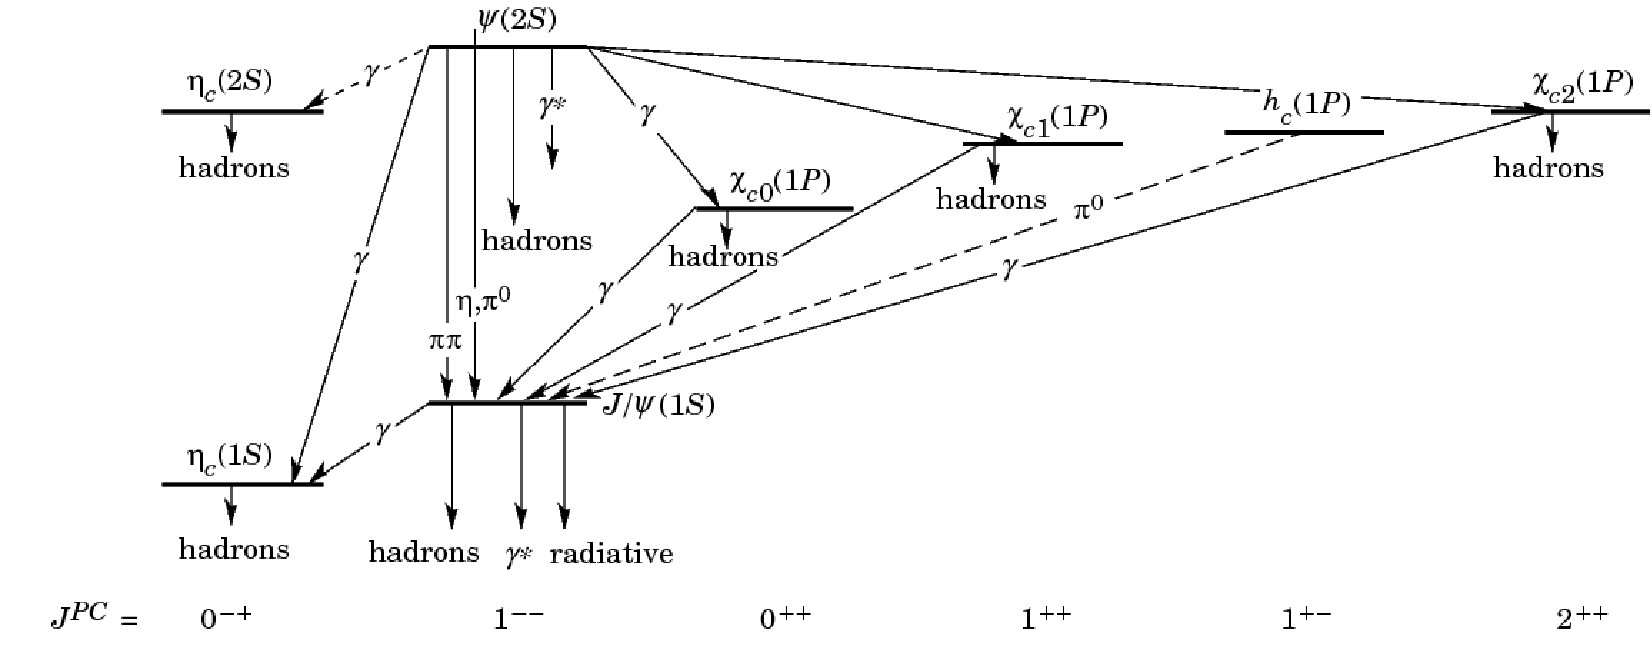
\includegraphics[width=\hugefigwidth]{chap_QuarkoniaSurvey_figures/JPsiFamily}
  \caption[J/$\psi$ family]
   {Different bound states of charm and anti-charm quark.}
   \label{fig:JPsiFamily}
\end{figure}



\begin{figure}
  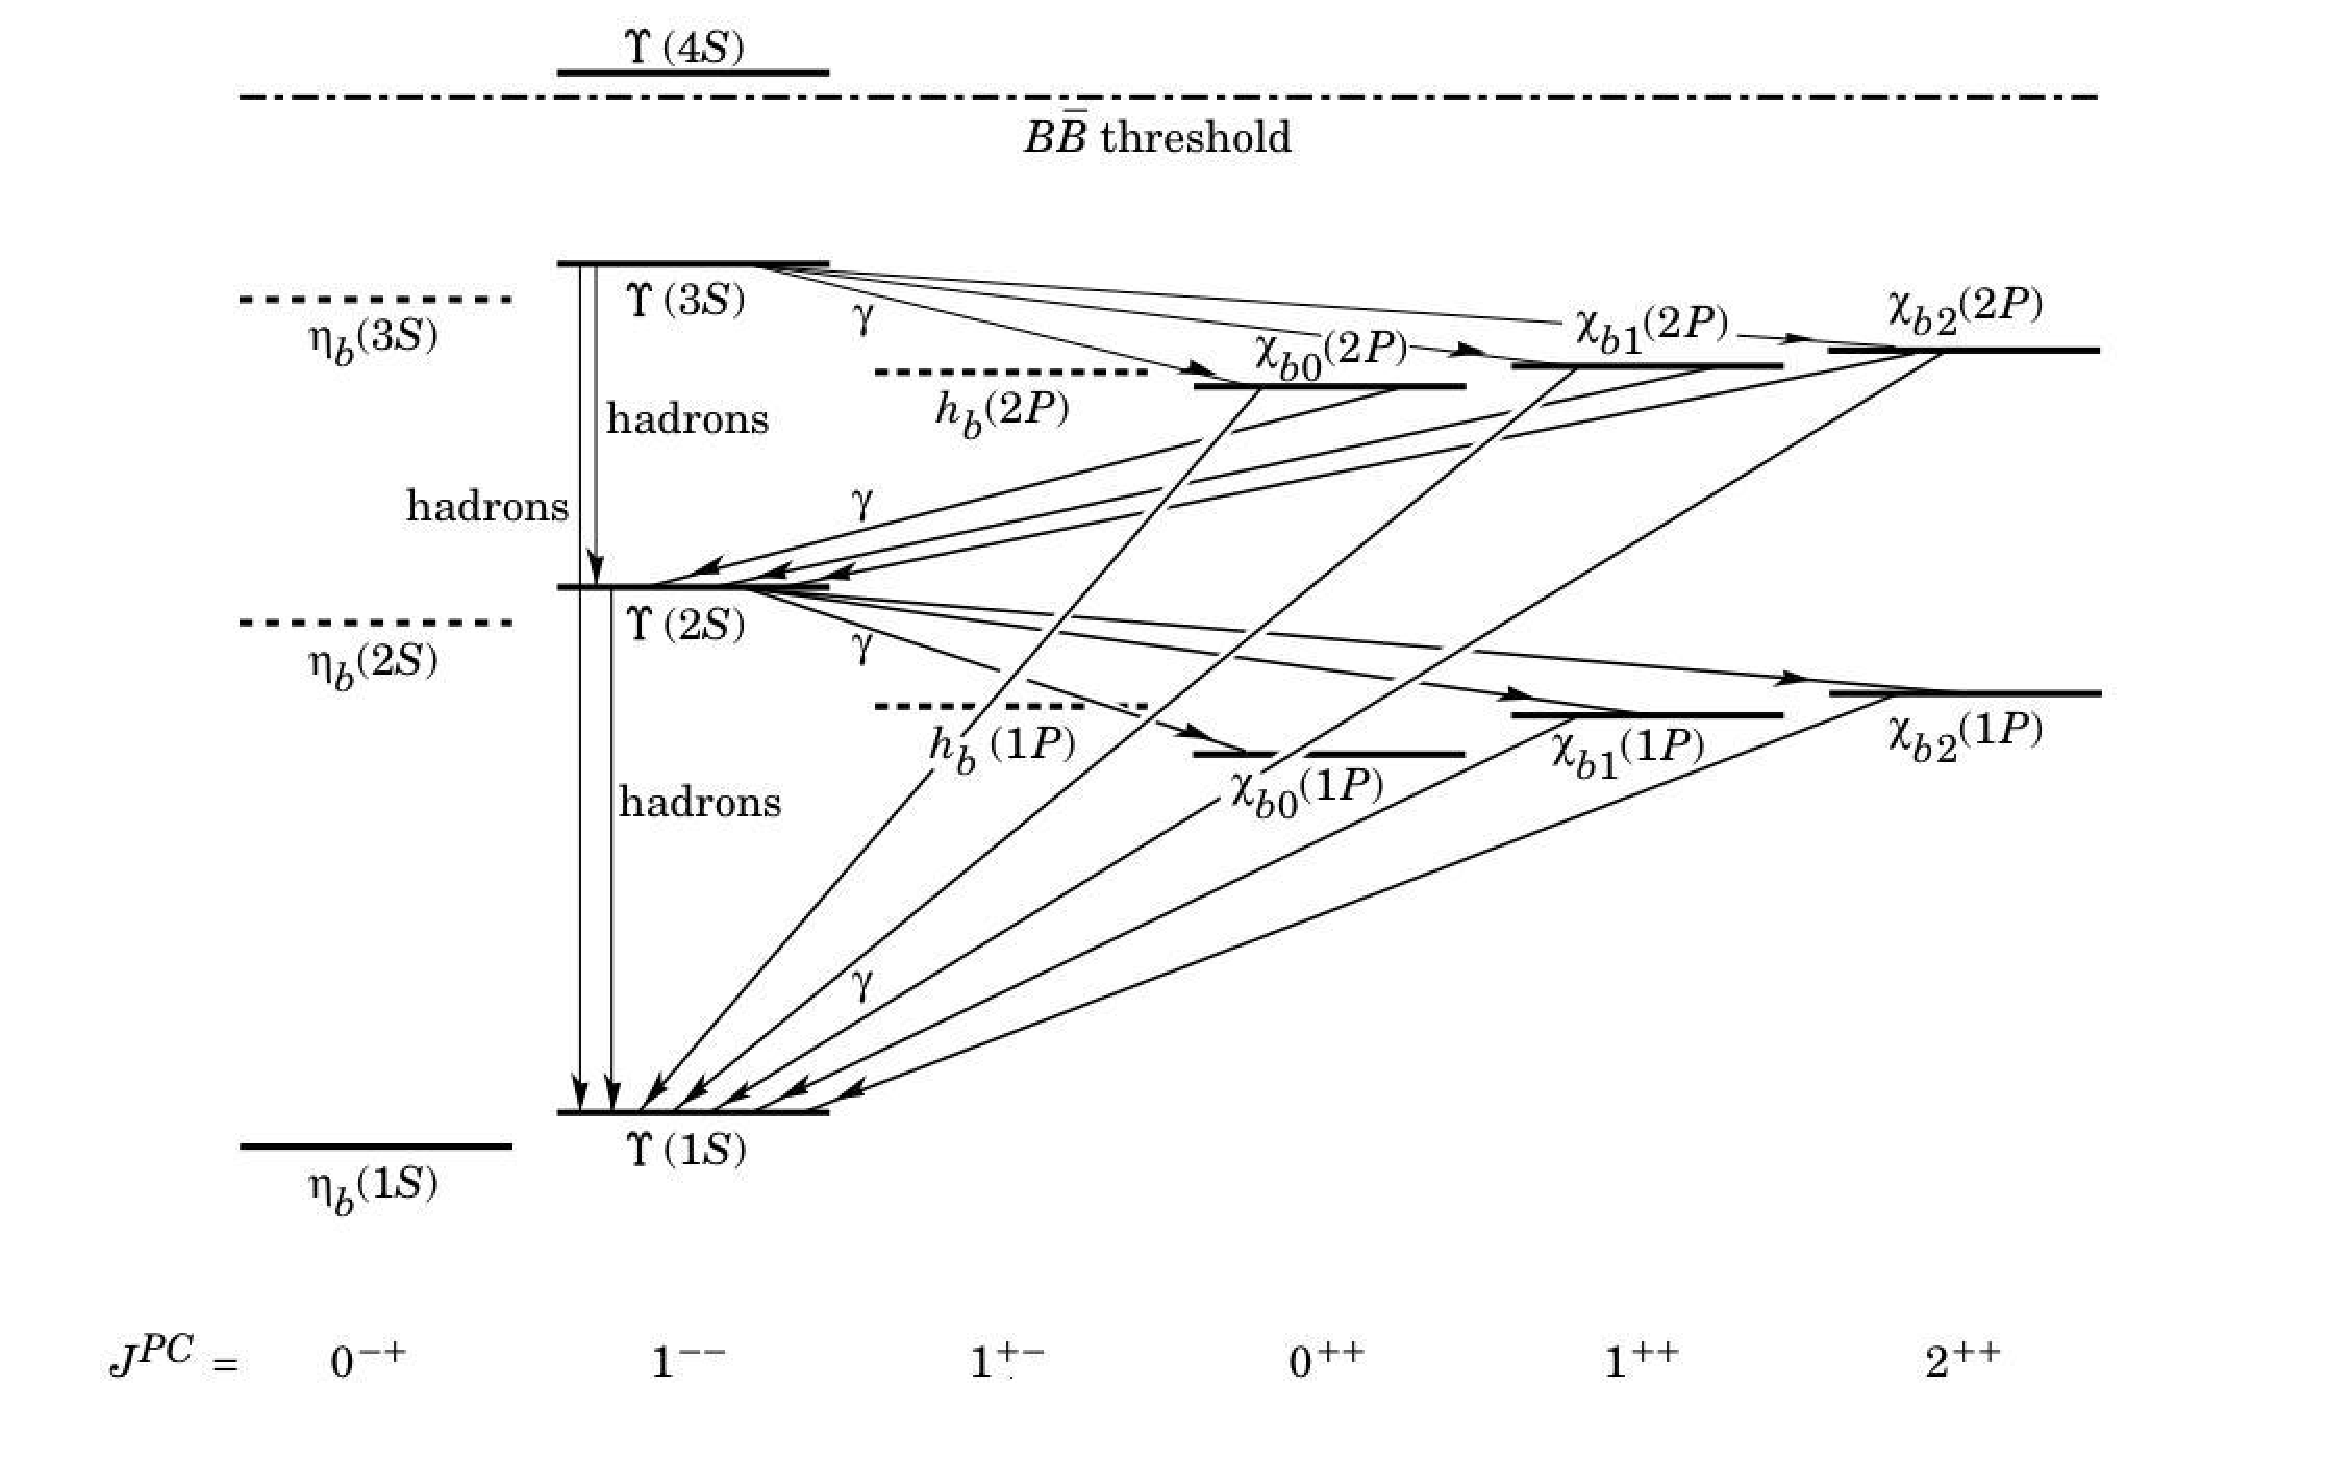
\includegraphics[width=\hugefigwidth]{chap_QuarkoniaSurvey_figures/UpsilonFamily}
  \caption[$\Upsilon$ family]
   {Different bound states of beauty and anti-beauty quark.}
   \label{fig:UpsilonFamily}
\end{figure}


\subsection{Quarkonium production}
In general one can subdivide the production process into two major parts
\begin{itemize}
\item Production of a heavy quark pair in hard collisions.
\item Formation of quarkonia out of the two heavy quarks.
\end{itemize}

{\bf Production of a heavy quark pair in hard collisions}\\
Due to the high mass of the heavy quarks (m$_{charm}\,\sim$ 1.3 GeV/c$^2$, m$_{bottom}\,\sim$ 4.7 GeV/c$^2$) 
the first process can happen only during the first phase of a collision. Only at that
time the elementary collisions with sufficiently high momentum transfers to
create such high masses take place. For this reason the heavy quark production
is a hard process that can be treated perturbatively. In next-to-leading order
(NLO) calculations the available experimental data at different energies and
collision system \cite{Baines,Ramona_Paper1} were described. The obtained parameters were then
used to predict the total production cross section in proton-proton collisions at
LHC energies. The charm production cross section is predicted to be 6.3 mb.
and the bottom production cross section 0.19 mb \cite{Ramona_Paper2}. To obtain upper and
lower limits for this cross sections the parameters have been varied leading to
a relatively large range for the charm production cross section of 4$-$15 mb and
0.08$-$0.34 mb for the bottom production cross section. \\
{\bf Formation of quarkonia out of the two heavy quarks}\\
The second part,namely the formation of quarkonia out of the quark-anti-quark pair can a
priori not be treated perturbative. Due to the high quark masses and the
small relative velocities in the quarkonium system, the formation can be described
using non-relativistic QCD (NRQCD). This allows the factorization
into a perturbative small-range and high-momentum part and a long-ranged
and low-momentum part. In the past years especially three models were developed,
namely the Color Singlet Model (CSM) \cite{CSM1, CSM2}, the Color Octet
Model \cite{COM1, COM2, COM3} and the Color Evaporation Model (CEM) \cite{CEM1, CEM2, CEM3}
\begin{itemize}
\item Color Singlet Model (CSM): The quarkonia formed out of the two quarks
has to be color neutral. Since in principal the two heavy quarks are not
necessarily carriers of one color and the corresponding anti-color, the
combination might be colored \footnotemark. The Color Singlet Model rejects all color

\footnotetext[1]{The symmetry group of QCD is the SU(3). The colors are triplet, R, G, B and their anti-color
$\overline{R},\overline{G}$ and $\overline{B}$  triplets one can form 3 $\bigotimes$ 3 = 8 $\bigoplus$ 1 
combinations, one octet and one singlet. The color octet states are R$\overline{G}$, R$\overline{B}$, 
G$\overline{R}$, G$\overline{B}$, B$\overline{R}$, B$\overline{G}$, 
$\sqrt{\frac{1}{2}}(R\overline{R}-G\overline{g})$, $\sqrt{\frac{1}{6}}(R\overline{R}+G\overline{G}-2B\overline{B})$,
. The color singlet is $\sqrt{\frac{1}{6}}(R\overline{R}+G\overline{G}+B\overline{B})$.}

octet states, in the NRQCD factorization the produced quarkonium has
the same quantum numbers as the quark$-$anti-quark pair. Predictions by
the CSM for the production of quarkonium in pp at Tevatron underestimated
the data by an order of magnitude, thus it was clear that the
color octet states cannot be neglected.

\item Color Octet Model (COM): The Color Octet model considers the octet
states, within the model quarkonium is only produced in an octet and
thus colored state. The pre$-$resonant colored state neutralizes its color
by the emission of a soft gluon. The Color Octet Model was able to
reproduce the production cross section but failed in the description of
the observed J/$\psi$  polarization \cite{CDF_Pola}.

\item Color Evaporation Model (CEM):As an expansion the Color Evaporation
Model was developed from the Color Octet Model. The evaporation of
the surplus color happens via many different processes, not only by the
emission of a soft gluon. This large number of processes results in a
relatively large number of parameters, that have to be determined by the
comparison to existing data. Although the tuning of the model to the
data works well, the large number of free parameters limit the predictive
power of the CEM. Nevertheless it is the best available approach for
describing the available measurements and it is used for the predictions
of the cross sections for LHC energies (see Figure \ref{fig:QuarkoniaCrossSection}).
\end{itemize}

\begin{figure}
  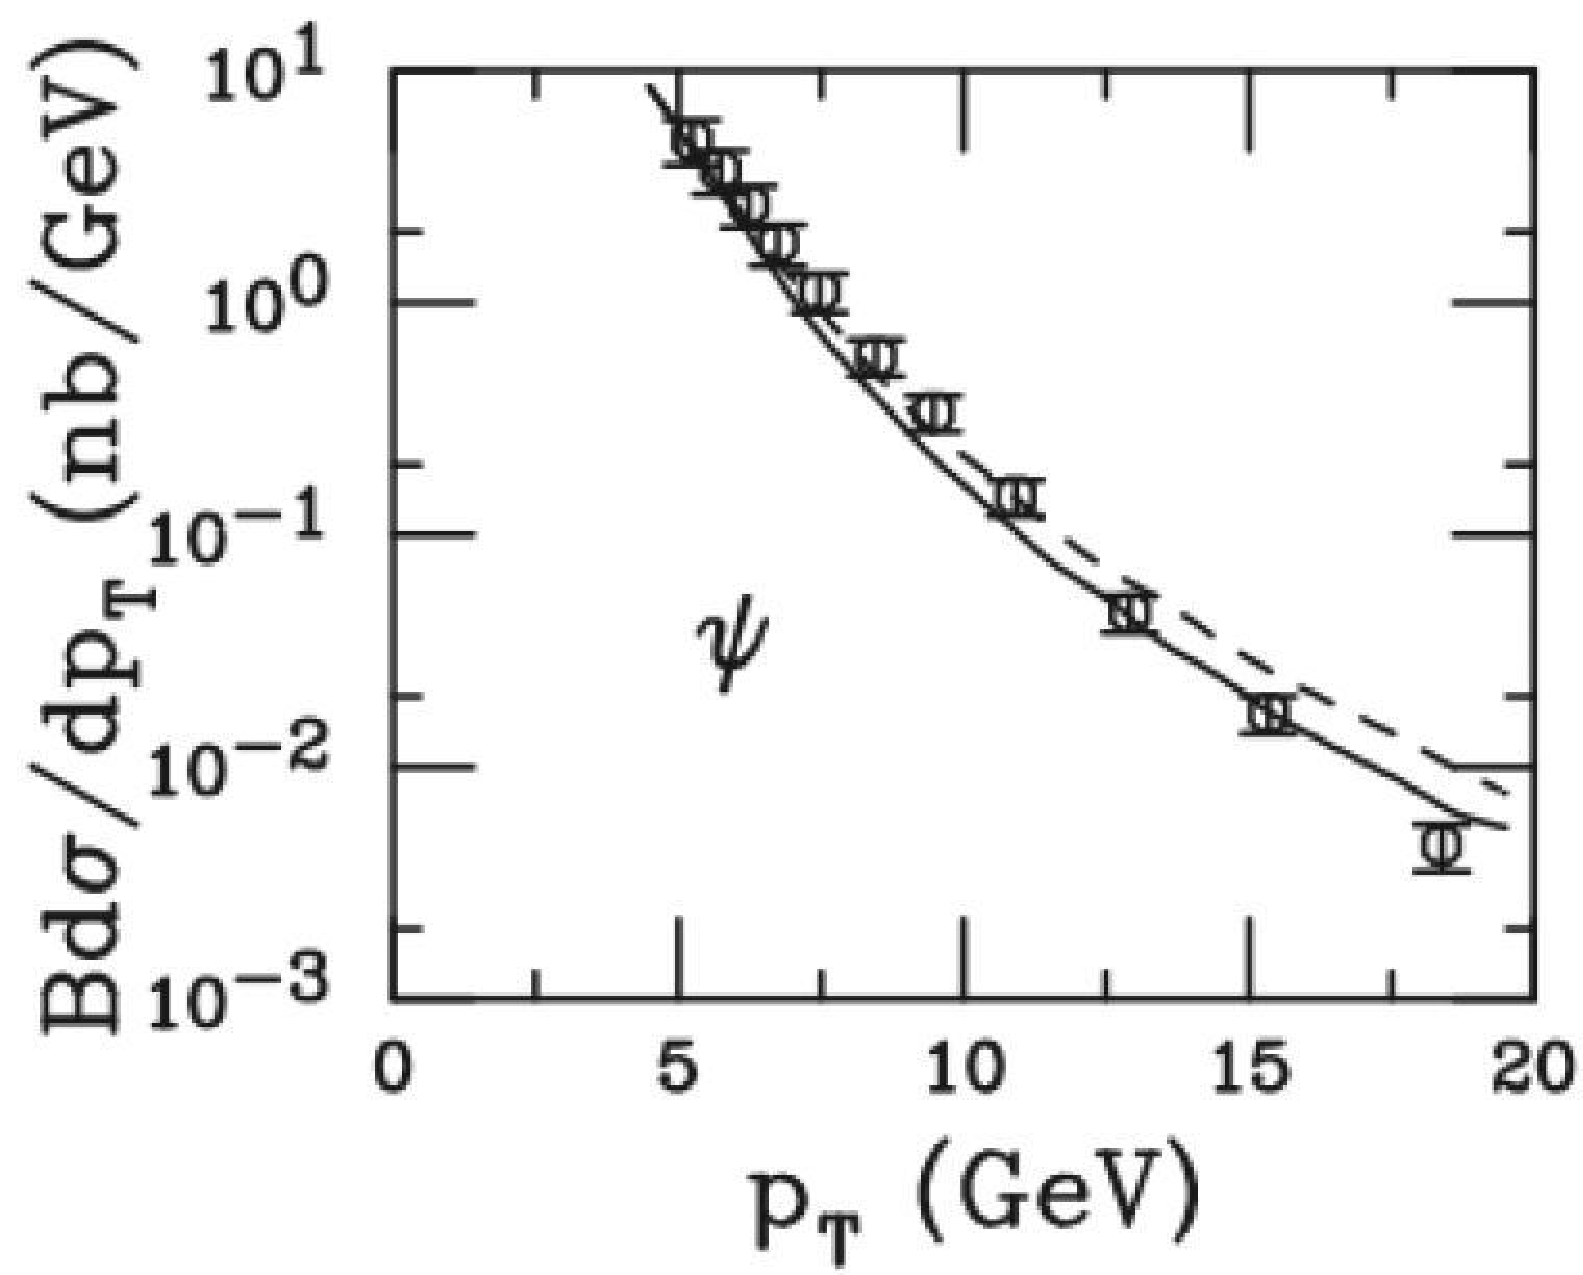
\includegraphics[width=\smallfigwidth]{chap_QuarkoniaSurvey_figures/JPsiCrossTevtron}
  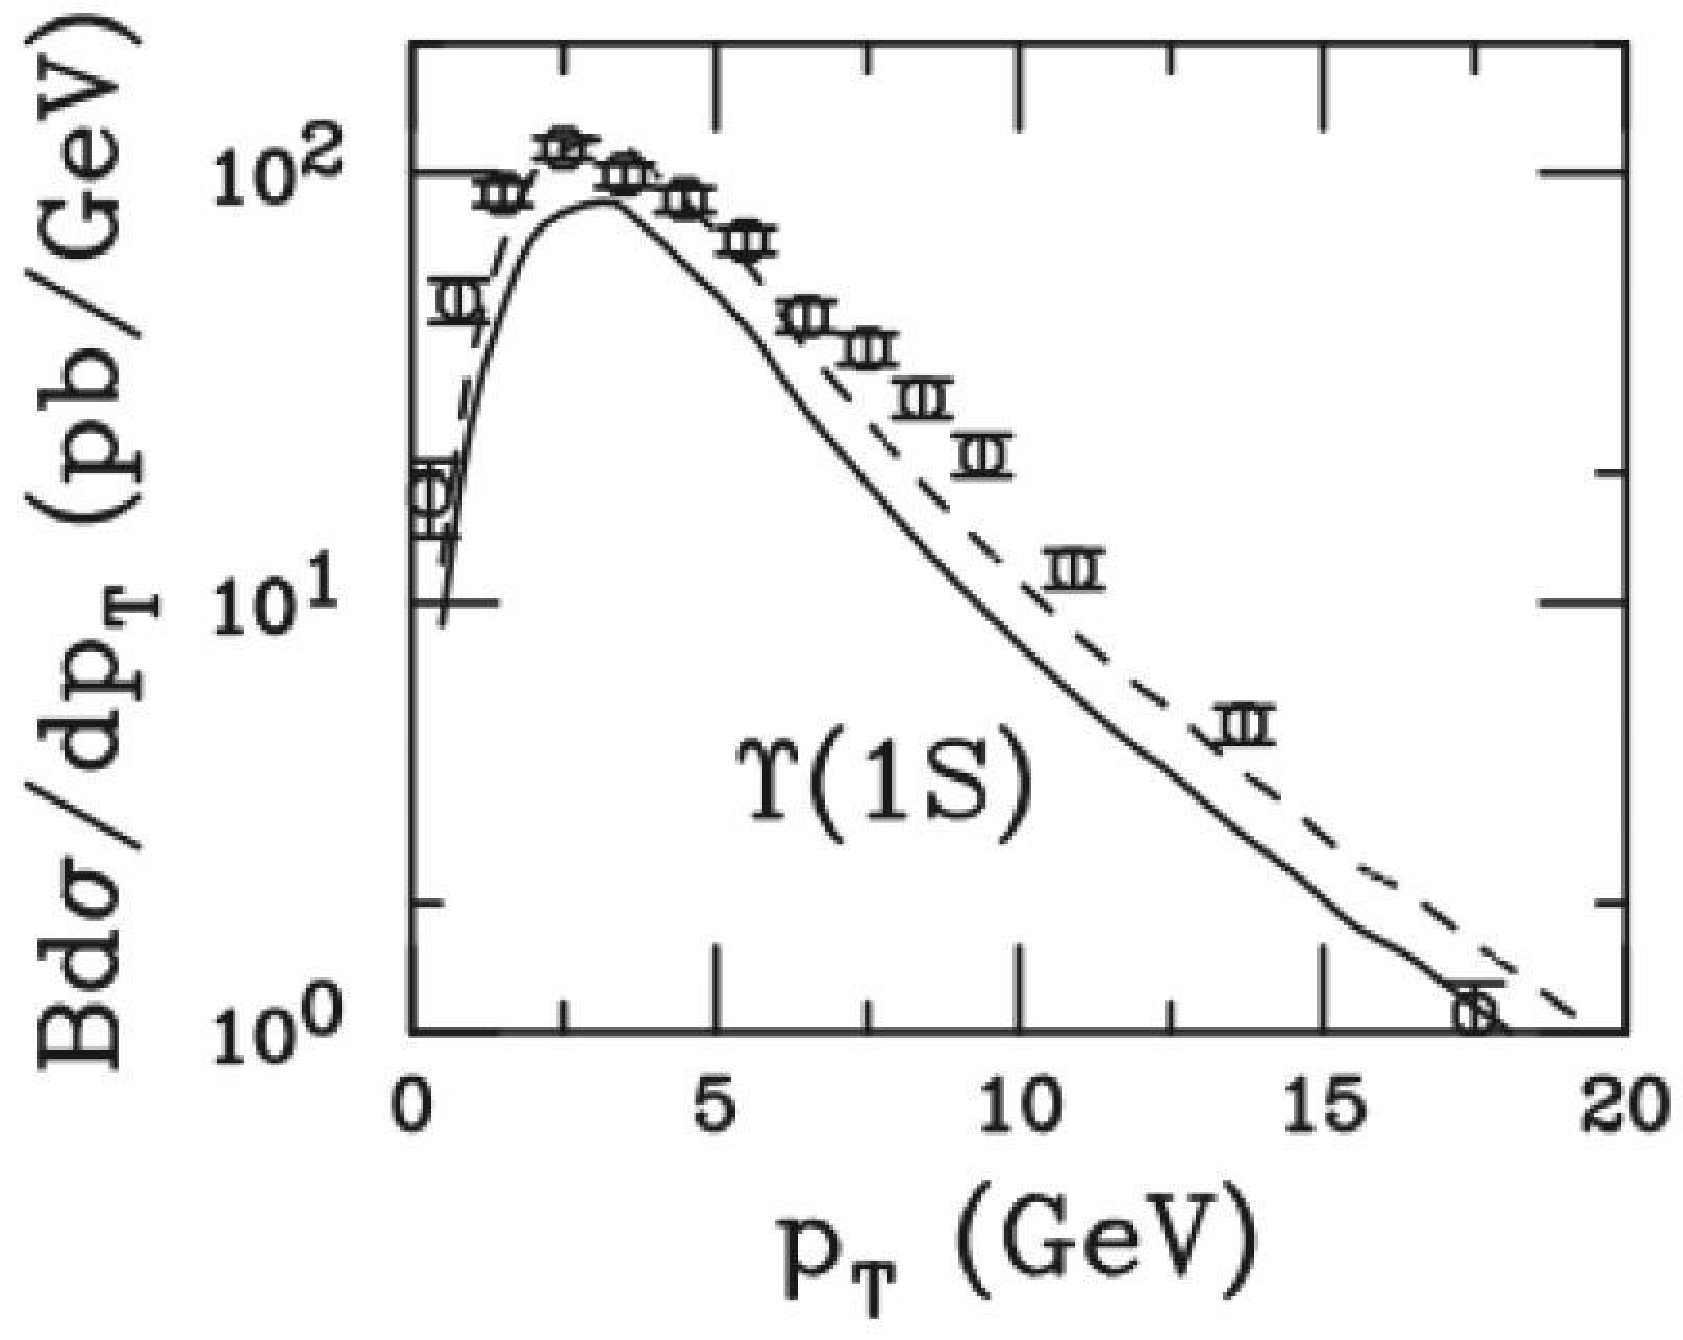
\includegraphics[width=\smallfigwidth]{chap_QuarkoniaSurvey_figures/YCrossTevtron}
  \caption[J/$\psi$ and $\Upsilon$ cross sections]
   {pT -dependent production of J/$\psi$ s and $\Upsilon$ s as measured by the
     CDF experiment \cite{CDF1, CDF2, CDF3} (circles) and compared to predictions by the
     Color Evaporation Model with two different parameter sets (solid+dotted).}
   \label{fig:QuarkoniaCrossSection}
\end{figure}



\subsection{Qualitative formation and decay times}
It is commonly accepted that at LHC energies the main production mechanism
of heavy quark and quarkonia is gluon fusion gg$\rightarrow$Q$\overline{Q}$. Gluons from the
nucleus wave function will form a Q$\overline{Q}$ pre$-$resonance in a characteristic (hard)
production time t$_p$
\begin{eqnarray}
t_p(p_t\, \gg\, m_Q) \approx \frac{E}{p_T^2} \approx \frac{1}{p_T},\,\,\,
t_p(p_t\, \leq\, m_Q)\sim \frac{1}{m_Q}
\end{eqnarray}
E being the pair energy. Thus, for p$_T \,\sim$ m$_Q$ the production time of
charm and beauty pre$-$resonance pairs would be about
\begin{eqnarray}
t_p(p_t\, \gg\, m_c) \sim 0.15 \mbox{fm/c},t_p(p_t\, \gg\, m_b) \sim 0.05 \mbox{fm/c}.   
\end{eqnarray}
The production time is then much smaller than 1 fm/c, and they are
formed at a relative distance 1/m$_Q\,\,\gg$ 1 fm. Then the Q$\overline{Q}$ pairs 
travel extremely close and to form a Q$\overline{Q}$ resonance they need to expand 
till the characteristic size of the resonance. It can be interpreted as the time 
the pair takes to decide which of the possible Q$\overline{Q}$ bound-states 
it will couple to (one with mass m1 or one with m2). This formation time can be calculated 
by means of \cite{Thews, Khar_Thews}
\begin{eqnarray}
t_f \simeq \frac{2E}{m_2^2 - m_1^2}
\end{eqnarray}

Thus the time a c$\overline{c}$ (b$\overline{b}$) pair takes to decide to form a J/$\psi$
($\Upsilon$) rather than a excited state

\begin{eqnarray}
t_f(J/\psi,E) \simeq \frac{2E}{m_{J/\psi}^2 - m_{\psi^{'}}^2} \nonumber \\
t_f(J/\psi,10 GeV) \simeq 1.0 fm/c.\nonumber \\
t_f(J/\psi,30 GeV) \simeq 3.0 fm/c. \nonumber \\
\end{eqnarray}

similarly for  $\Upsilon$ family

\begin{eqnarray}
t_f(\Upsilon,E) \simeq \frac{2E}{m_{\Upsilon}^2 - m_{\Upsilon^{'}}^2} \nonumber \\
t_f(\Upsilon,10 GeV) \simeq 0.36 fm/c.\nonumber \\
t_f(\Upsilon,30 GeV) \simeq 1.1 fm/c. \nonumber \\
\end{eqnarray}

The resonances formation times are thus much larger than the preresonances
production times. They increase with the particle momentum,
ranging from a fraction of fm/c to about 3 fm/c.
Later, the Q$\overline{Q}$ resonance being not a stable particle, it will decay with
a characteristic proper time inversely proportional to its width
\begin{eqnarray}
t_d \simeq \frac{1}{\Gamma}
\end{eqnarray}
The J/$\psi$  and $\Upsilon$ decay time would then be of about

\begin{eqnarray}
t_d(J/\psi) \simeq \frac{1}{93 keV} = 2.1\times10^{3} fm/c, \,\,\,
t_d(\Upsilon) \simeq \frac{1}{54 keV} = 3.7\times10^{3} fm/c.
\end{eqnarray}

Theoretical calculations estimate that at LHC energies the QGP might
be formed in about 0.1 fm/c and might last $\geq$ 10 fm/c. The previous calculations
suggest that: the Q$\overline{Q}$ pre$-$resonances are produced while the QGP is
formed, but the Q$\overline{Q}$ resonances are formed in coexistence with the QGP, and
may decay out of it.

\subsection{Quarkonium binding potential}
Since heavy quarks are massive, quarkonium spectroscopy can be studied in
non$-$relativistic quantum mechanics. The confining potential for a Q$\overline{Q}$ pair 
at a separation distance r can be modeled by \cite{SATZ, SATZ2}
\begin{eqnarray}
V_{Q\overline{Q}} &= \sigma(T)-\frac{\alpha_{eff}}{r} \\
\end{eqnarray}
where $\sigma\,\simeq$ 0.216 GeV$^2$ is the string tension (for T $\sim $0), and 
$\alpha_{eff}\,\,\simeq\,\frac{\pi}{12}$  accounts for the Coulombian-like interaction. 
At small distances (r small), the Coulombian-like interaction is predominant, 
whereas at large distances the attractive force of the confinement described by the 
string tension prevails.
The latter increasing linearly with the distance, a big amount of energy would
be needed to separate the heavy quarks, they are tightly bound. Above T$_C$
quarks and gluons are no longer confined and the large color charge present
in the medium screens the inter-quark potential, the so called color screening.
The potential is then expected to be described by a Debye-screening form
\begin{eqnarray}
V_{Q\overline{Q}}^{QGP} (r,T) &= -\frac{\alpha_{eff}}{r}e^{-\frac{r}{\lambda_D(T)}}
\end{eqnarray}
$\lambda_D$(T) being the Debye screening length.  $\lambda_D$(T) diminishing with the
system temperature, the inter$-$quark potential is reduced accordingly, and when
 $\lambda_D$(T) $\leq$ r$_{hadron}$ the inter$-$quark force can not hold the quarks together, 
and they dissociate.

\begin{figure}
  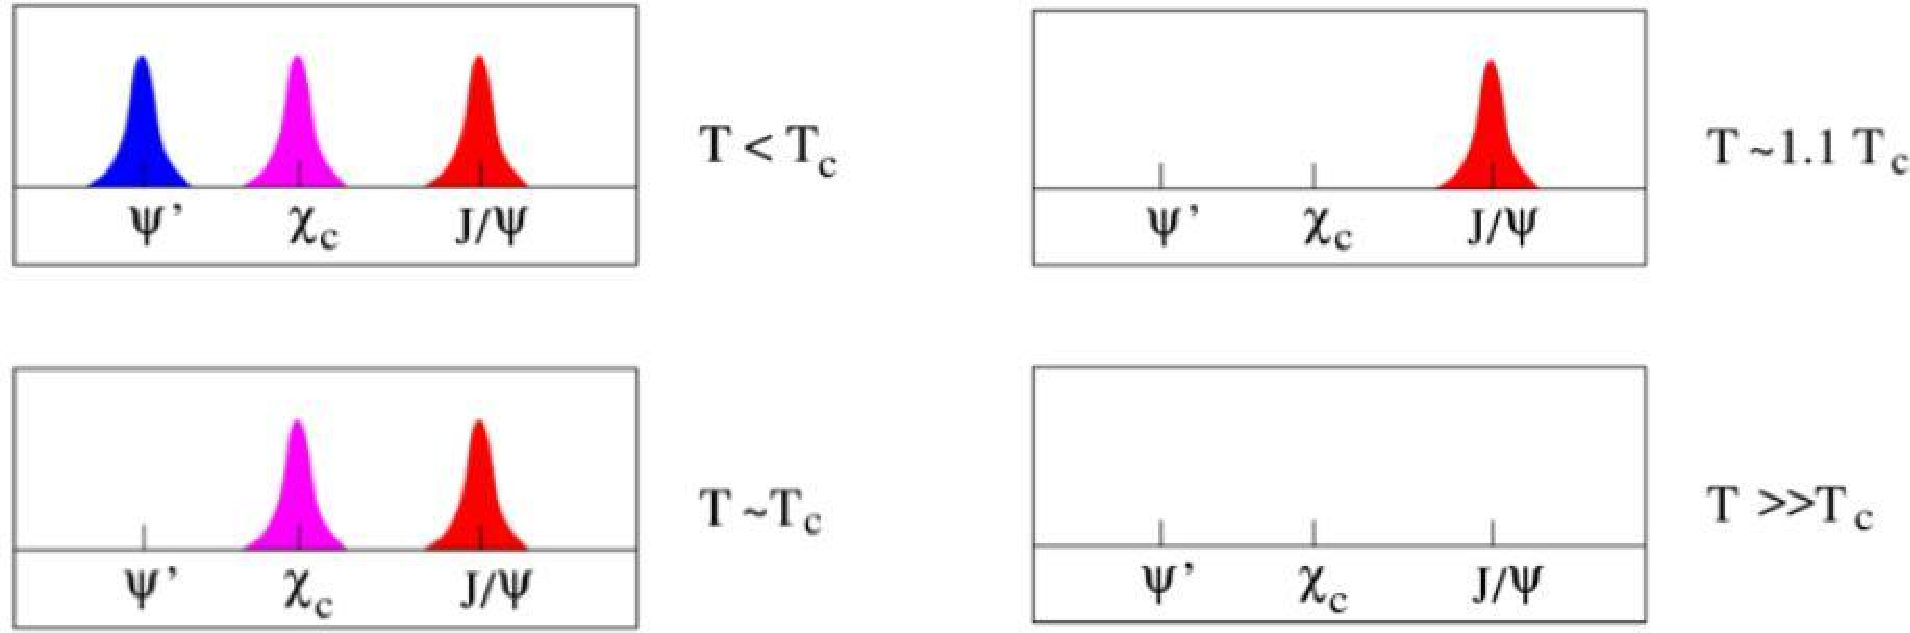
\includegraphics[width=\hugefigwidth]{chap_QuarkoniaSurvey_figures/Quarkonia_SATZ2}
  \caption[QuarkoniaAtTc]{Charmonium spectra at different temperatures \cite{SATZ2}.}
   \label{fig:QuarkoniaAtTc}
\end{figure}



LQCD can give accurate estimates of the quarkonium binding potential
as a function of the system temperature and the inter$-$quark separation
r in the relativistic limit. Such calculations allow them to predict the dissociation
temperatures T$_d$ of the quarkonium states. Table \ref{tab:quarkoniaproperties} summarizes
the results obtained by using the full internal energy (including the entropy
term) \cite{SATZ,Frithjof}. An illustration of the situation for the charmonium dissociation
temperatures is displayed in Figure \ref{fig:QuarkoniaAtTc}. A ``sequential melting'' pattern of the
various charmonium states with their binding energy is observed, the ground
state disappearing the last. Recent LQCD calculations support the late dissociation
of J/$\psi$($\Upsilon$) at about T$_d$/T$_c$ = 1.5(3.2) \cite{Matthias} in agreement with LQCD
spectral analysis of the hadron correlation functions \cite{Jakovac}.

\begin{table}[bht]
\caption[QuarkoniaProperties]{Dissociation temperatures of the quarkonium resonances from
LQCD. Where E$_b$ stands for the binding energy \cite{SATZ, Rev_PartPhysics, Frithjof}.}
\label{tab:quarkoniaproperties}
\begin{tabular}{lllllllll}
\hline
               &J/$\psi$(1S)  &$\chi_c$(1P)  &$\psi^{1}$(2S)  &$\Upsilon(1S)$  &$\chi_b$(1P)  &$\Upsilon$(2S)  &$\chi_b$(2P)  &$\Upsilon$(3S) \\
\hline
M[GeV]             &3.10          &3.41          &3.69           &9.46            &9.86           &10.02          &10.23         &10.36  \\              
E$_b$[GeV]         &0.64          &0.20          &0.05           &1.10            &0.67           &0.54           &0.31          &0.20   \\
$\frac{T_d}{T_c}$  &2.1           &1.16          &1.12            &$\geq$4.0      &1.76           &1.60           &1.19          &1.17   \\
\hline
\end{tabular}
\end{table}


\section{Experimental Status of Quarkonia Suppression}

\subsection{J/$\psi$ anomalous suppression at SPS}
A first J/$\psi$  suppression was observed and reported by the NA38 experiment
\cite{NA38}, which was performed with oxygen-uranium collisions of incident energy
200 GeV per nucleon. Figure \ref{fig:JPsiAtSPSNA38} shows the measured J/$\psi$  yield normalized
to the number of dimuons in mass range 2.7$-$3.5 GeV/c$^2$ as a function of transverse
energy (E$_T$ ) corresponded to centrality. A similar pattern was observed
later in sulphur-uranium collisions \cite{NA50}. Increasing centrality, the nuclear matter
is more and more compressed, at some point a volume of deconfined matter
forms with free color charges. Charmonium binding potential is screened and
the bound state is dissolved and then the measured J/$\psi$  production decreases
with respect to the reference. Because the ratio would be expected to remain
constant with respect to the centrality if charmonium is not suppressed.
However, another trial of explanation is possible without deconfinement
for the charmonium dissociation. It can be happened in the interactions with
nucleons. As pointed out in \cite{Khar_Carlos} the observed suppression is able to be presented
by the breakup of charmonium caused by scattering off nucleons, where
the matter is confined. The experiment of smaller system such as proton$-$nucleus
or deuterium$-$nucleus collisions was designed to examine this effect,
namely nuclear absorption. Indeed the effect of nuclear absorption was measured,
absorption cross section as $\sigma_{\mbox{abs}}$ = 7.3$\pm$0.6 mb \cite{Khar_Carlos}. 
The NA50 experiment compared the charmonium production to the Drell-Yan (q$\overline{q}\rightarrow l^+l^-$) 
process, since the compete dimuon continuum in the J/$\psi$  mass range can not be predicted
from theory \cite{NA51}. Figure \ref{fig:JPsiAtSPS} illustrates the ratio of J/$\psi$  and Drell$-$Yan
process as a function of L, the length of traversed nuclear matter, which can
be obtained from Glauber model calculation \cite{Khar_Carlos,NA51_2}. Thus the line shows the
amount of suppression due to nuclear absorption, that can not be related to
the dissociation from deconfinement. A clear deviation from this line can be
observed for L $>$ 7.5 fm. This suppression is called the anomalous suppression.

To determine the energy density necessary to melt charmonium, measurements on smaller 
systems have been performed. Although the maximum achievable energy density is smaller 
than in collisions of larger nuclei, smaller systems enable a higher resolution centrality 
scan. The results are shown in Figure \ref{fig:JPsiAtSPSNA50} (left) \cite{Scomparin}. 
The J/$\psi$/Drell-Yan production is plotted as a function of
the number of participants in the collision, where the data is normalized to cold
matter effects. A suppression exceeding the nuclear suppression is seen starting from 80 
participants on. In Figure \ref{fig:JPsiAtSPSNA50} (right) the data is compared to the
results of the NA50 experiments from lead-lead collisions of the same energy of
158 GeV per nucleon. For peripheral collisions the ratio of measured/expected
J/$\psi$ yield is as expected, close to one, any observed dissociation is attributed
to cold nuclear effects. For more central collisions a clear deviation from the
expected behavior is observed, with good agreement between the In$-$In and the
Pb$-$Pb data
The measurement of $\psi^{'}$ has been performed as shown in Figure \ref{fig:PsiAtSPSNA50NA60}. All
the measurements suffer from the significantly lower statistics accumulated
for the $\psi^{'}$, because it is not only due to the lower production cross section,
but dominantly due to the lower branching into dileptons ($\sigma_{\psi^{'}} \rightarrow l^{+}l^{-}= 0.73 \%$
compared to $\sigma_{J/\psi} \rightarrow l^{+}l^{-}= 5.9 \%$ ).
Figure \ref{fig:PsiAtSPSNA50NA60} presents the similar suppression of $\psi^{'}$ is observed compared to
the J/$\psi$ only the onset of the anomalous suppression is already at L = 4fm
and thus happens at a lower energy density.

\subsection{J/$\psi$ and $\Upsilon(nS)$ suppression at RHIC}
At RHIC J/$\psi$ yield in AA collisions is compared with scaled yield in p+p collisions. 
It gives a new varibale known as Nuclear Modification Factor or R$_{AA}$.
\begin{eqnarray}
R_{AA} &= \frac{1}{N_{Coll}} \frac{\frac{d^{2}N^{J/\Psi}_{AA}}{dy dp_{T}}}{ \frac{d^{2}N^{J/\Psi}_{pp}}{dy dp_{T}}} \\
\end{eqnarray}

\subsubsection{J/$\psi$ suppression at PHENIX}
Figure \ref{fig:JPsiAtPHENIX1} shows the suppression pattern observed by PHENIX in Au$-$
Au and Cu$-$Cu collisions. The suppression of J/$\psi$  is observed in the more
central collisions. Since cold nuclear matter effects are not subtracted here the
observed suppression can not be attributed to the dissociation of quarkonia in
the deconfined medium alone. Figure \ref{fig:JPsiAtPHENIX2} presents the ratio of R$_{AA}$ and cold
nuclear matter effects (CNM) \cite{Phenix1}. For the comparison to previous results, the
J/$\psi$  data taken by NA50 and NA60 are included. The data agree quite well
between SPS and RHIC in the lower energy densities, while the suppression
observed at RHIC clearly exceeds the maximal suppression measured at SPS
of R$_{AA}$/CNM = 60 $\%$ in the higher energy densities

In particular, PHENIX measured R$_{AA}$ at different rapidity region. 
Figure \ref{fig:JPsiAtPHENIX2} illustrates J/$\psi$  R$_{AA}$ in four different centrality bins 
as a function of rapidity. While R$_{AA}$ is almost constant for peripheral collisions 
(centrality bins 40-60 $\%$ and 60-92 $\%$), the central collisions show a clear 
difference between forward and mid rapidity. The suppression of J/$\psi$  production is 
significantly lower in forward/backward direction compared to the observed suppression
at mid rapidity. This phenomenon could so far not be explained by current
quarkonia production and suppression models.


\begin{figure}
  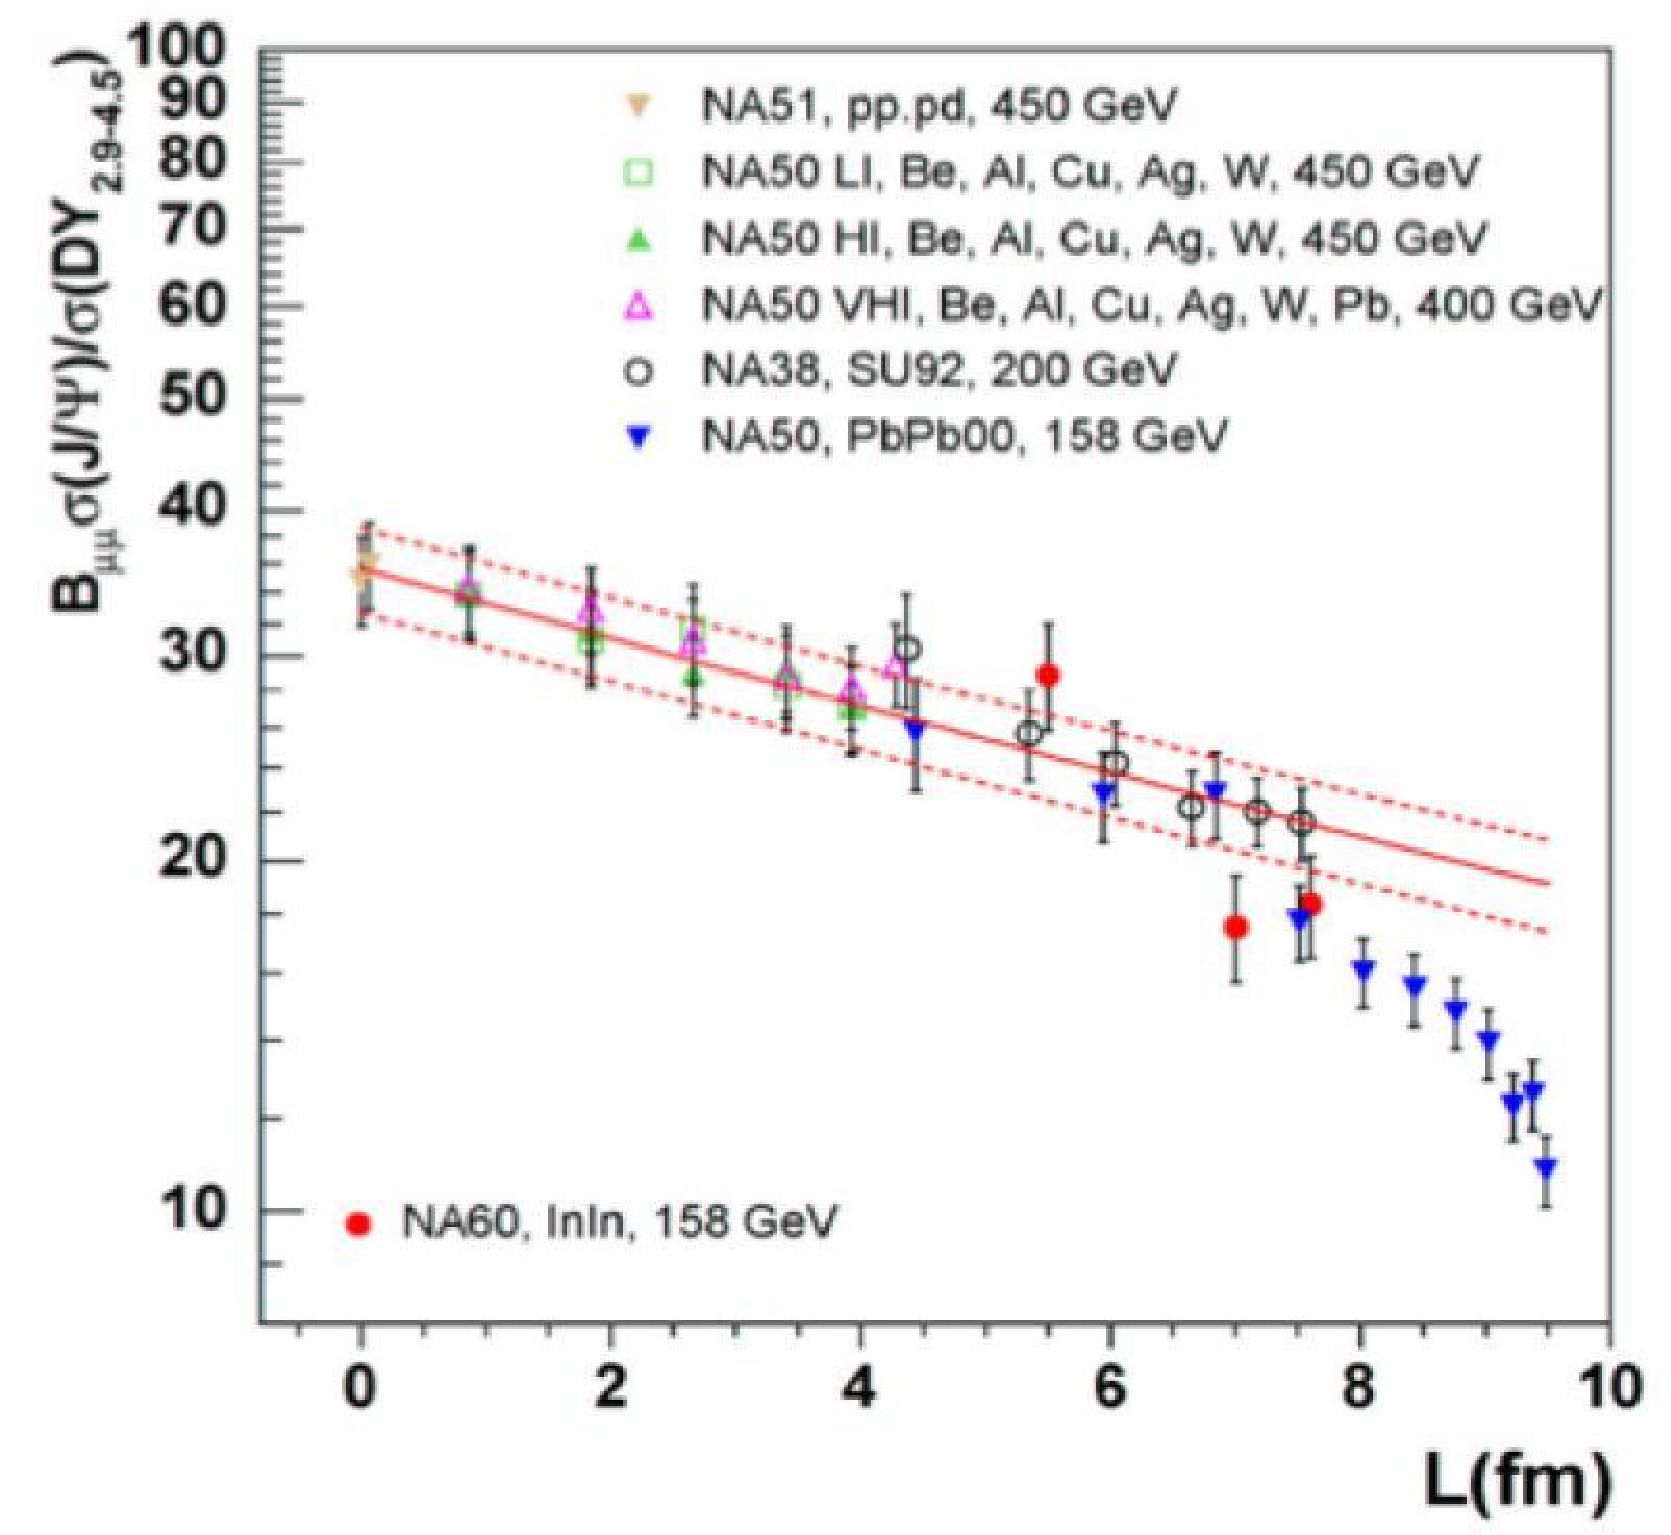
\includegraphics[width=\largefigwidth]{chap_QuarkoniaSurvey_figures/SPSNA51_27}
  \caption[JPsiAtSPSCrossSection]{J/$\psi$ over Drell$-$Yan production cross$-$section ratio as a function
of the length traversed by the charmonium in nuclear matter (L) for various colliding systems \cite{Pillot}.}
   \label{fig:JPsiAtSPS}
\end{figure}


\begin{figure}
  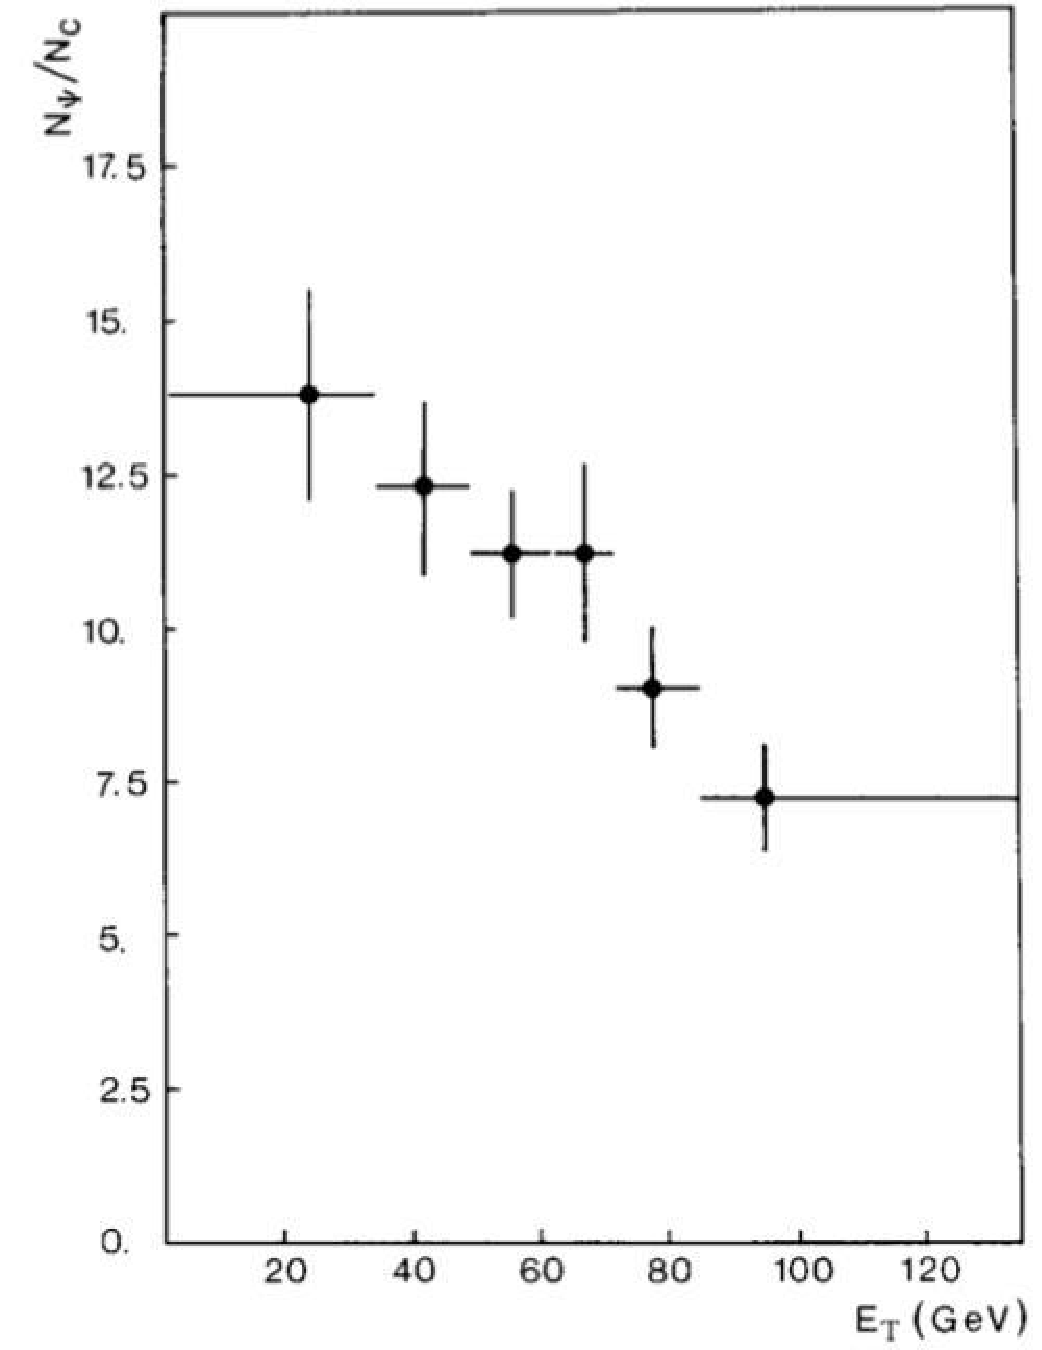
\includegraphics[width=\largefigwidth]{chap_QuarkoniaSurvey_figures/SPS_216}
  \caption[JPsiNA38]{The ratio of produced J/$\psi$  and dimuons as a function of the transverse energy as measured by NA38 \cite{NA38}.}
   \label{fig:JPsiAtSPSNA38}
\end{figure}



\begin{figure}
  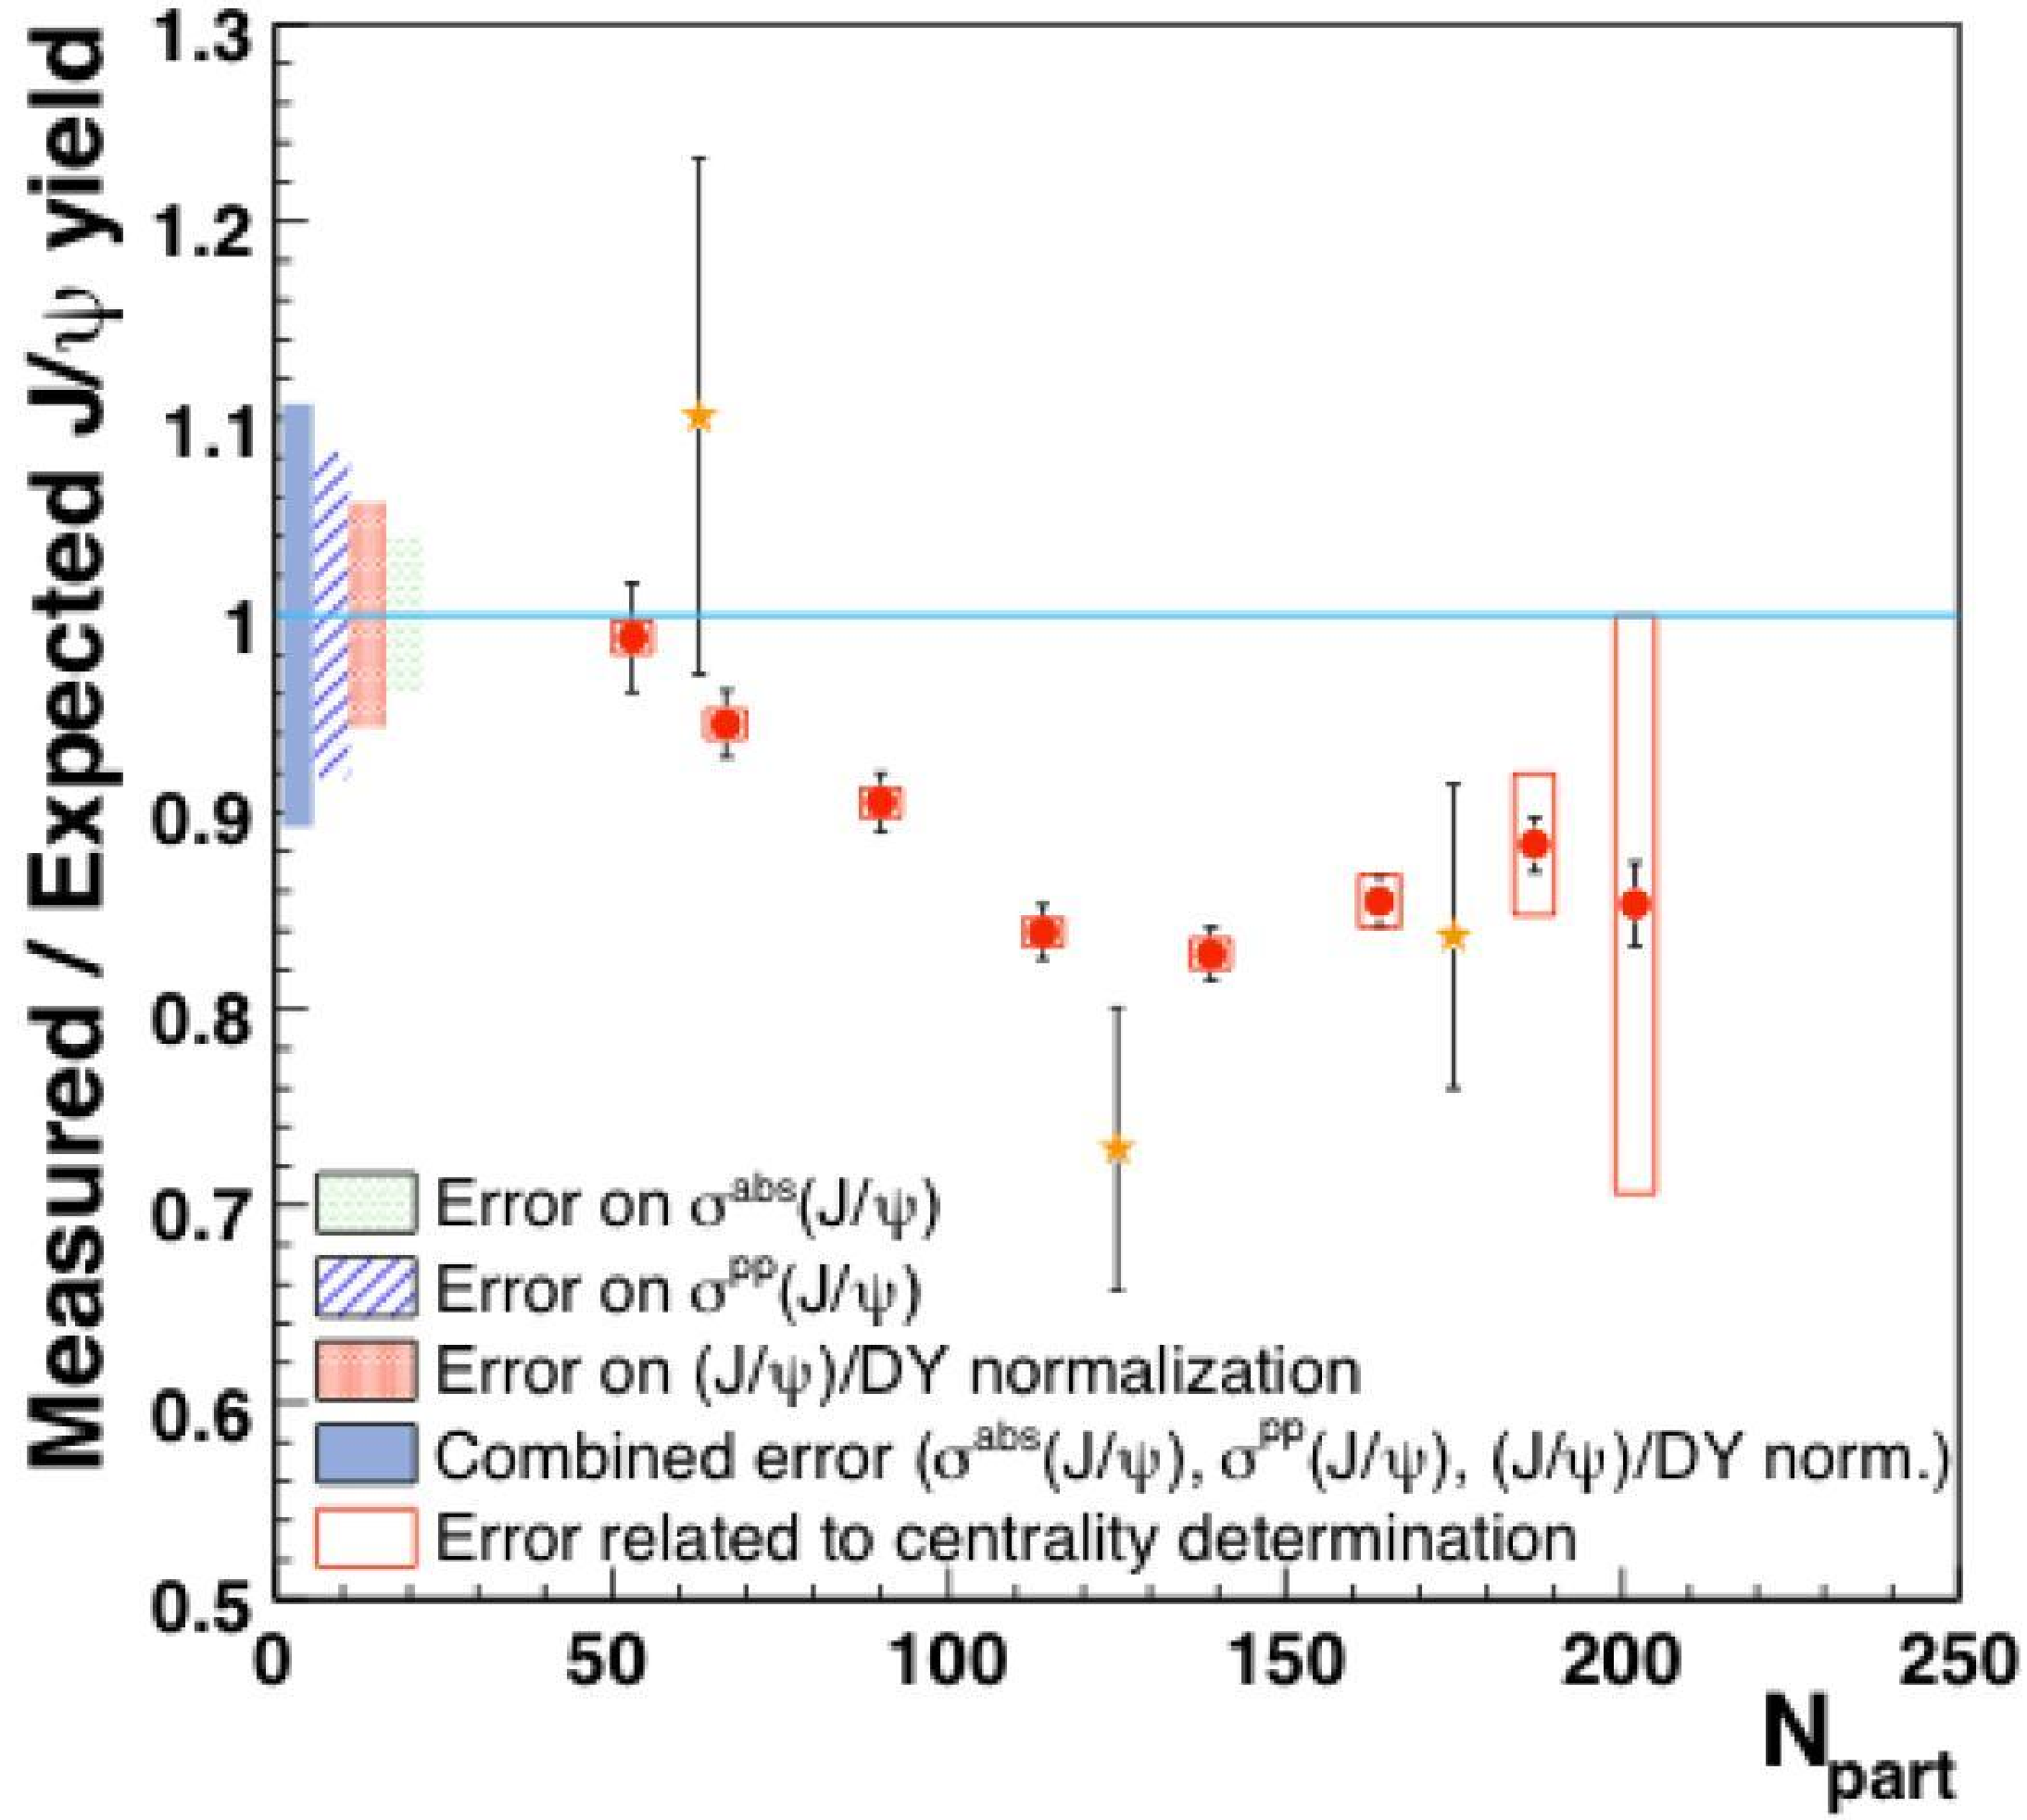
\includegraphics[width=\smallfigwidth]{chap_QuarkoniaSurvey_figures/SPS_217_1}
  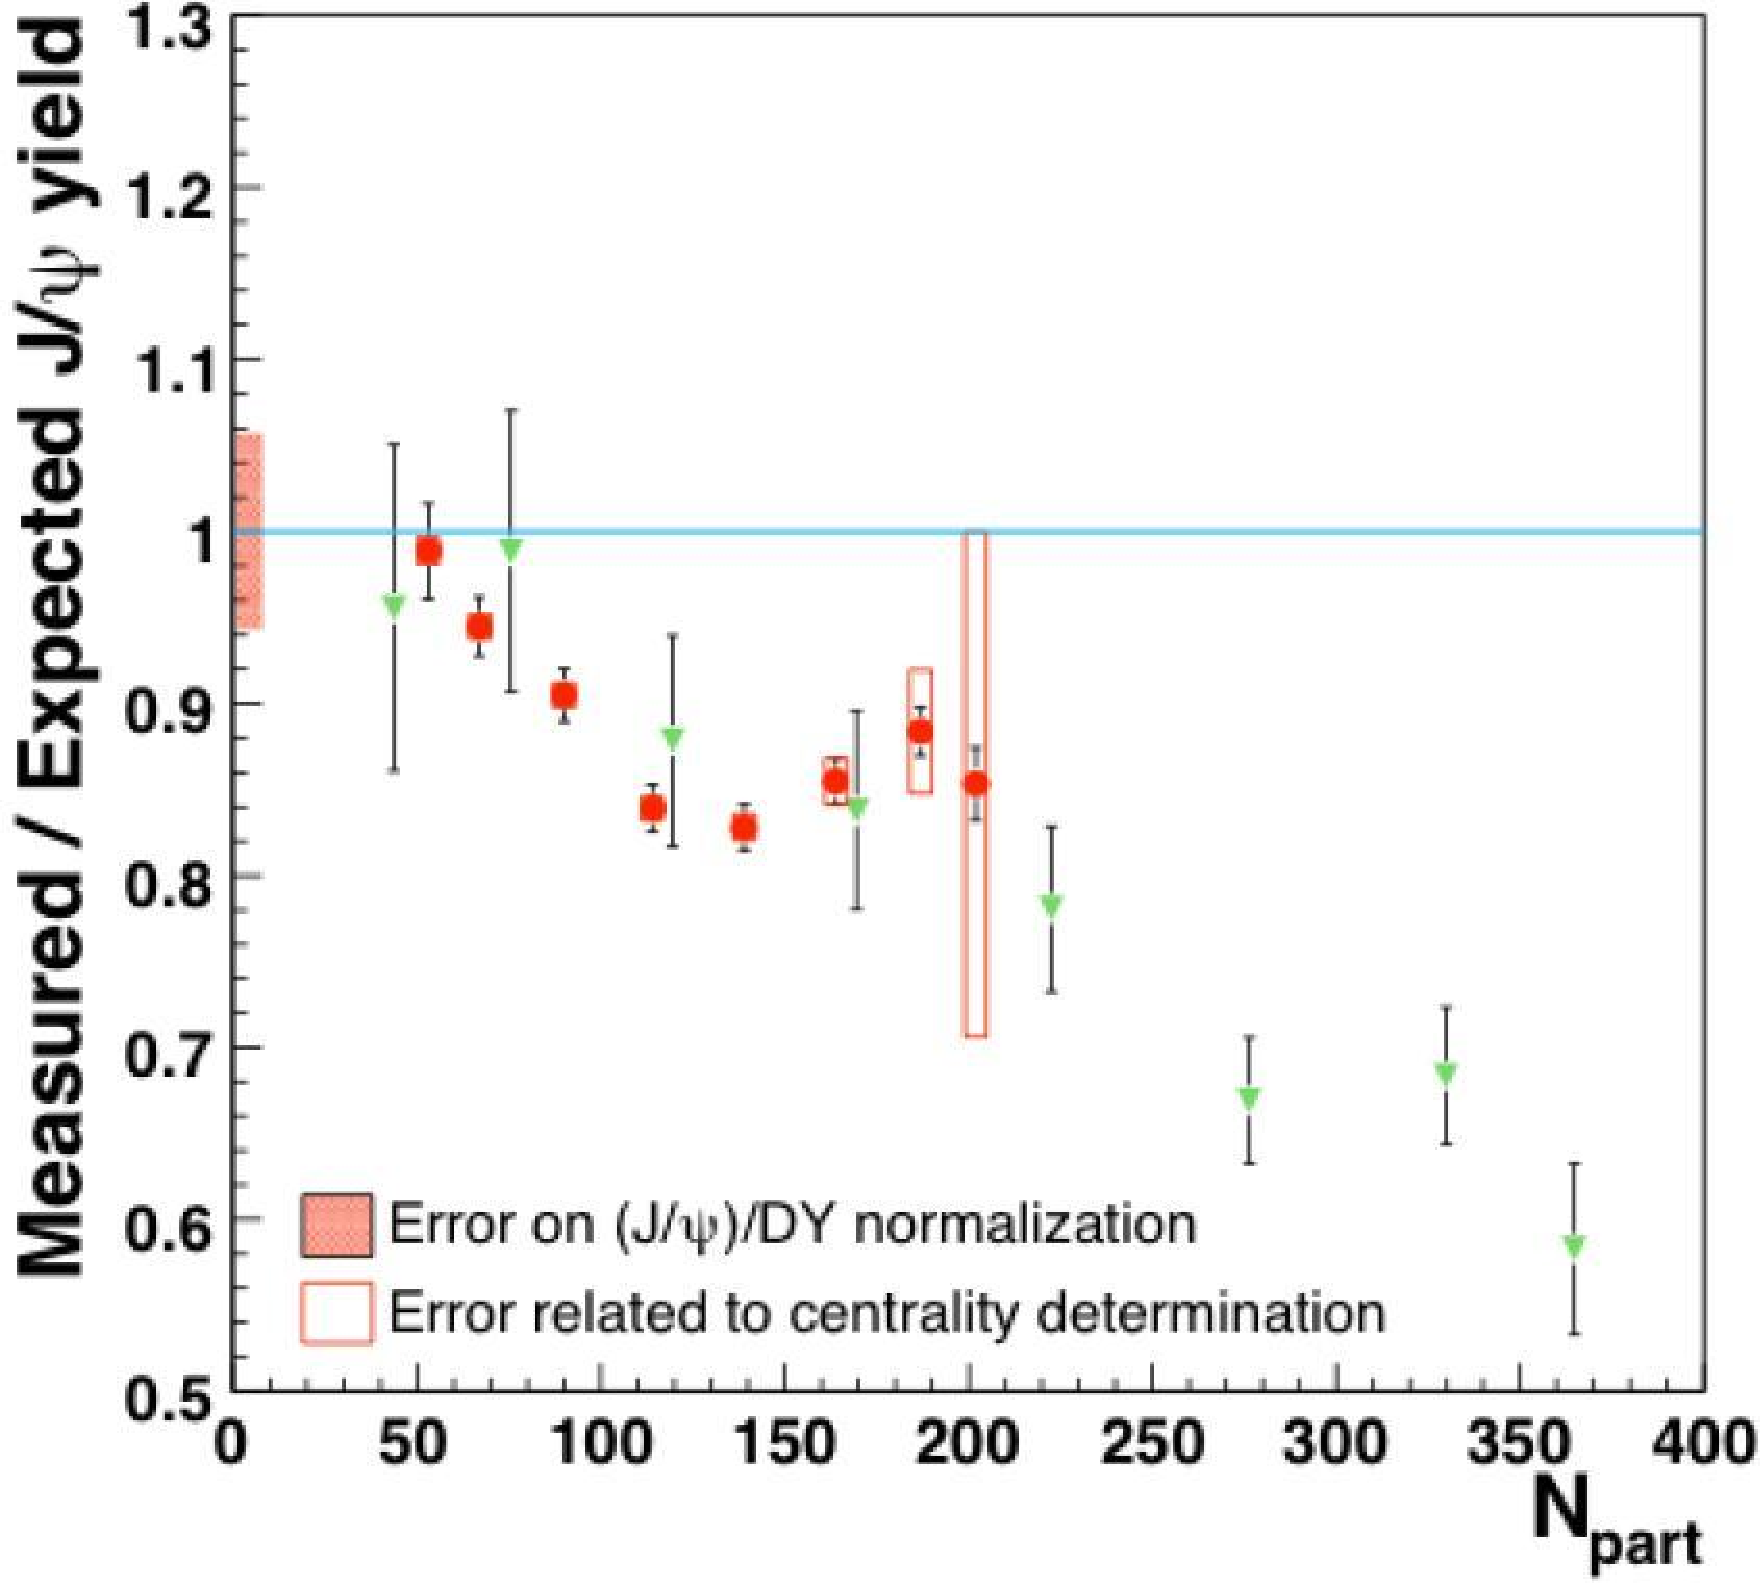
\includegraphics[width=\smallfigwidth]{chap_QuarkoniaSurvey_figures/SPS_217_2}
  \caption[JPsiNA50]{The centrality dependence of the J/$\psi$  suppression for In$-$In collisions at 158 GeV per nucleon measured by NA60 (left). 
    A comparison between the NA60 In$-$In and the NA50 Pb-Pb data (right).}
  \label{fig:JPsiAtSPSNA50}
\end{figure}




\begin{figure}
  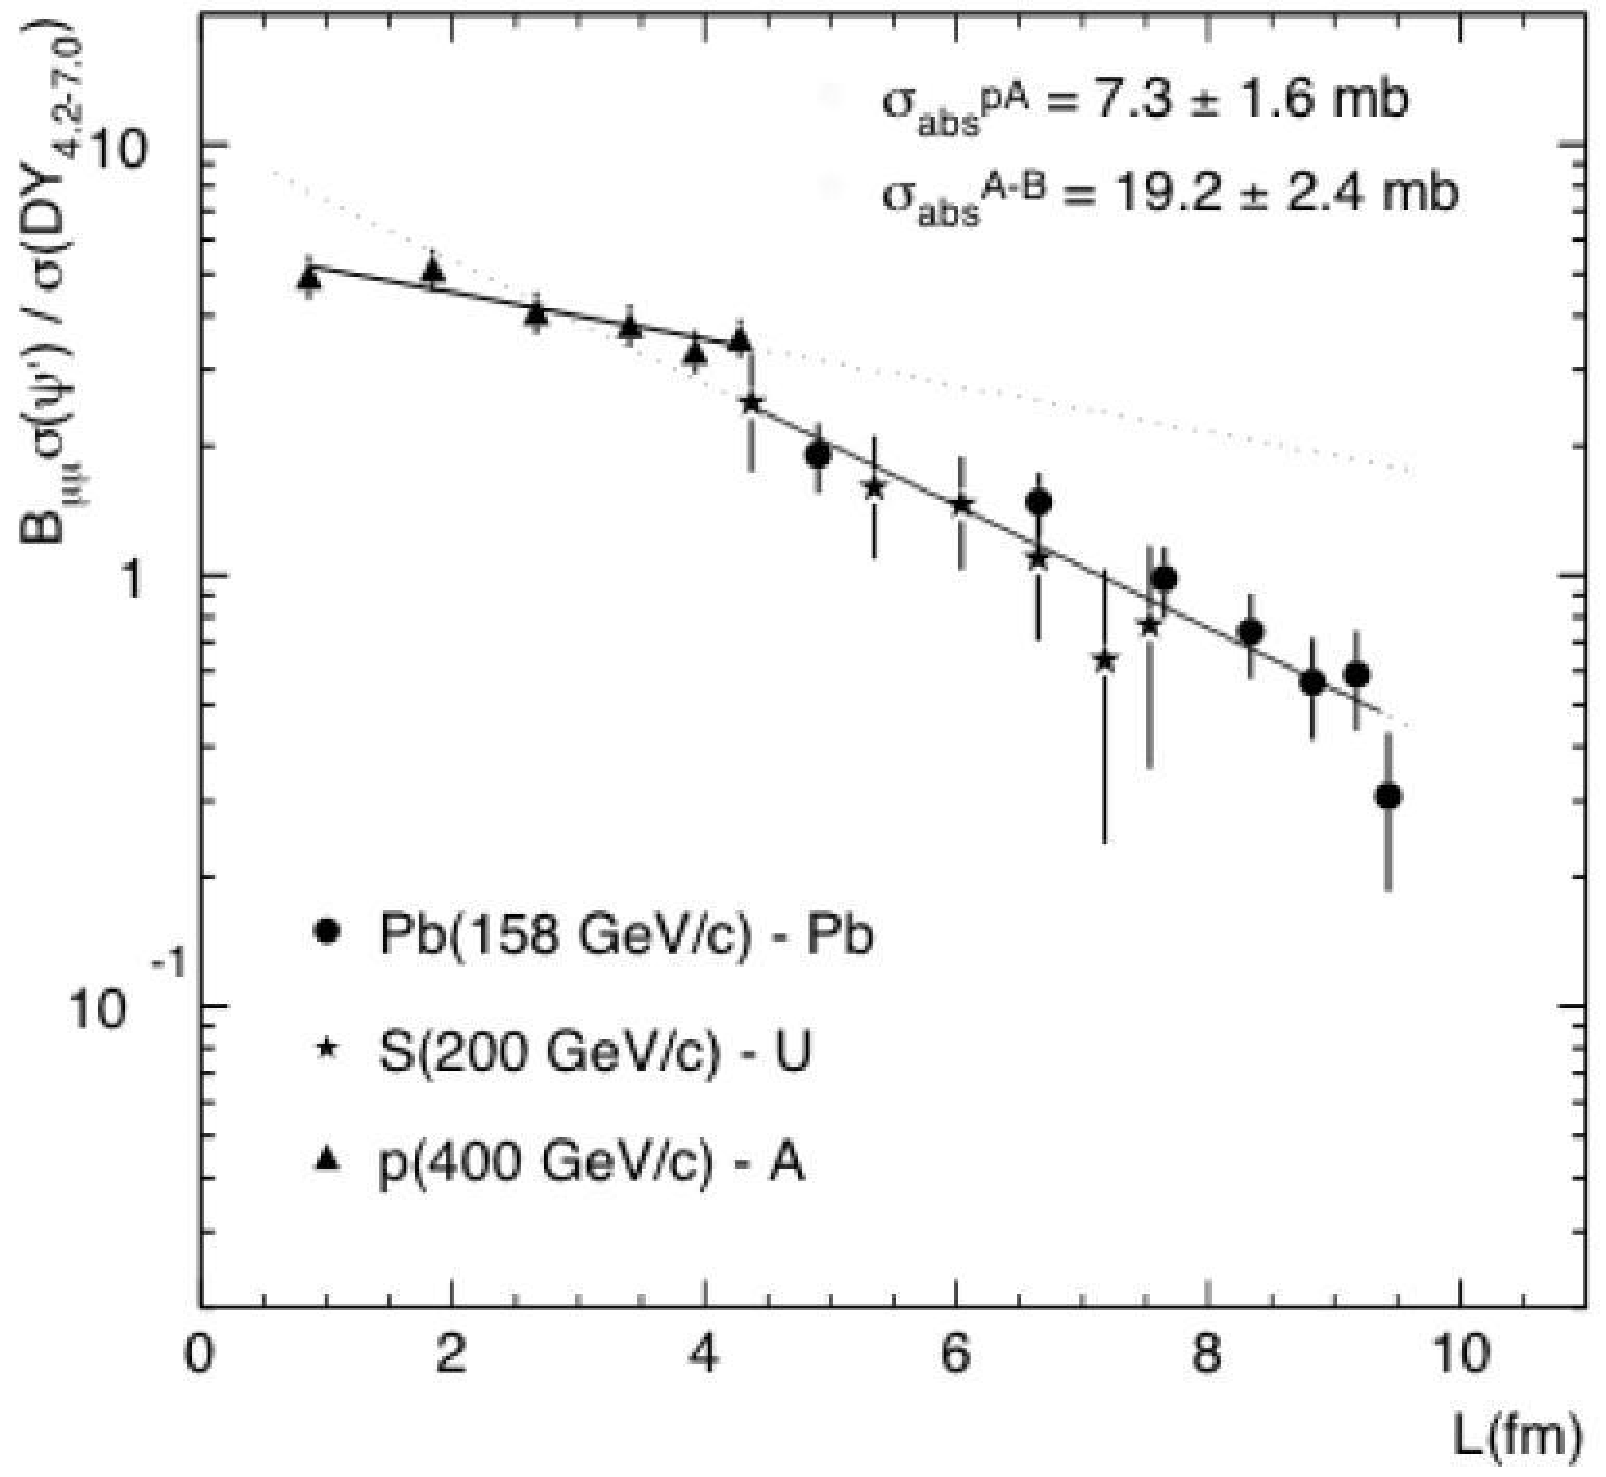
\includegraphics[width=\smallfigwidth]{chap_QuarkoniaSurvey_figures/SPS_Psi_218_1}
  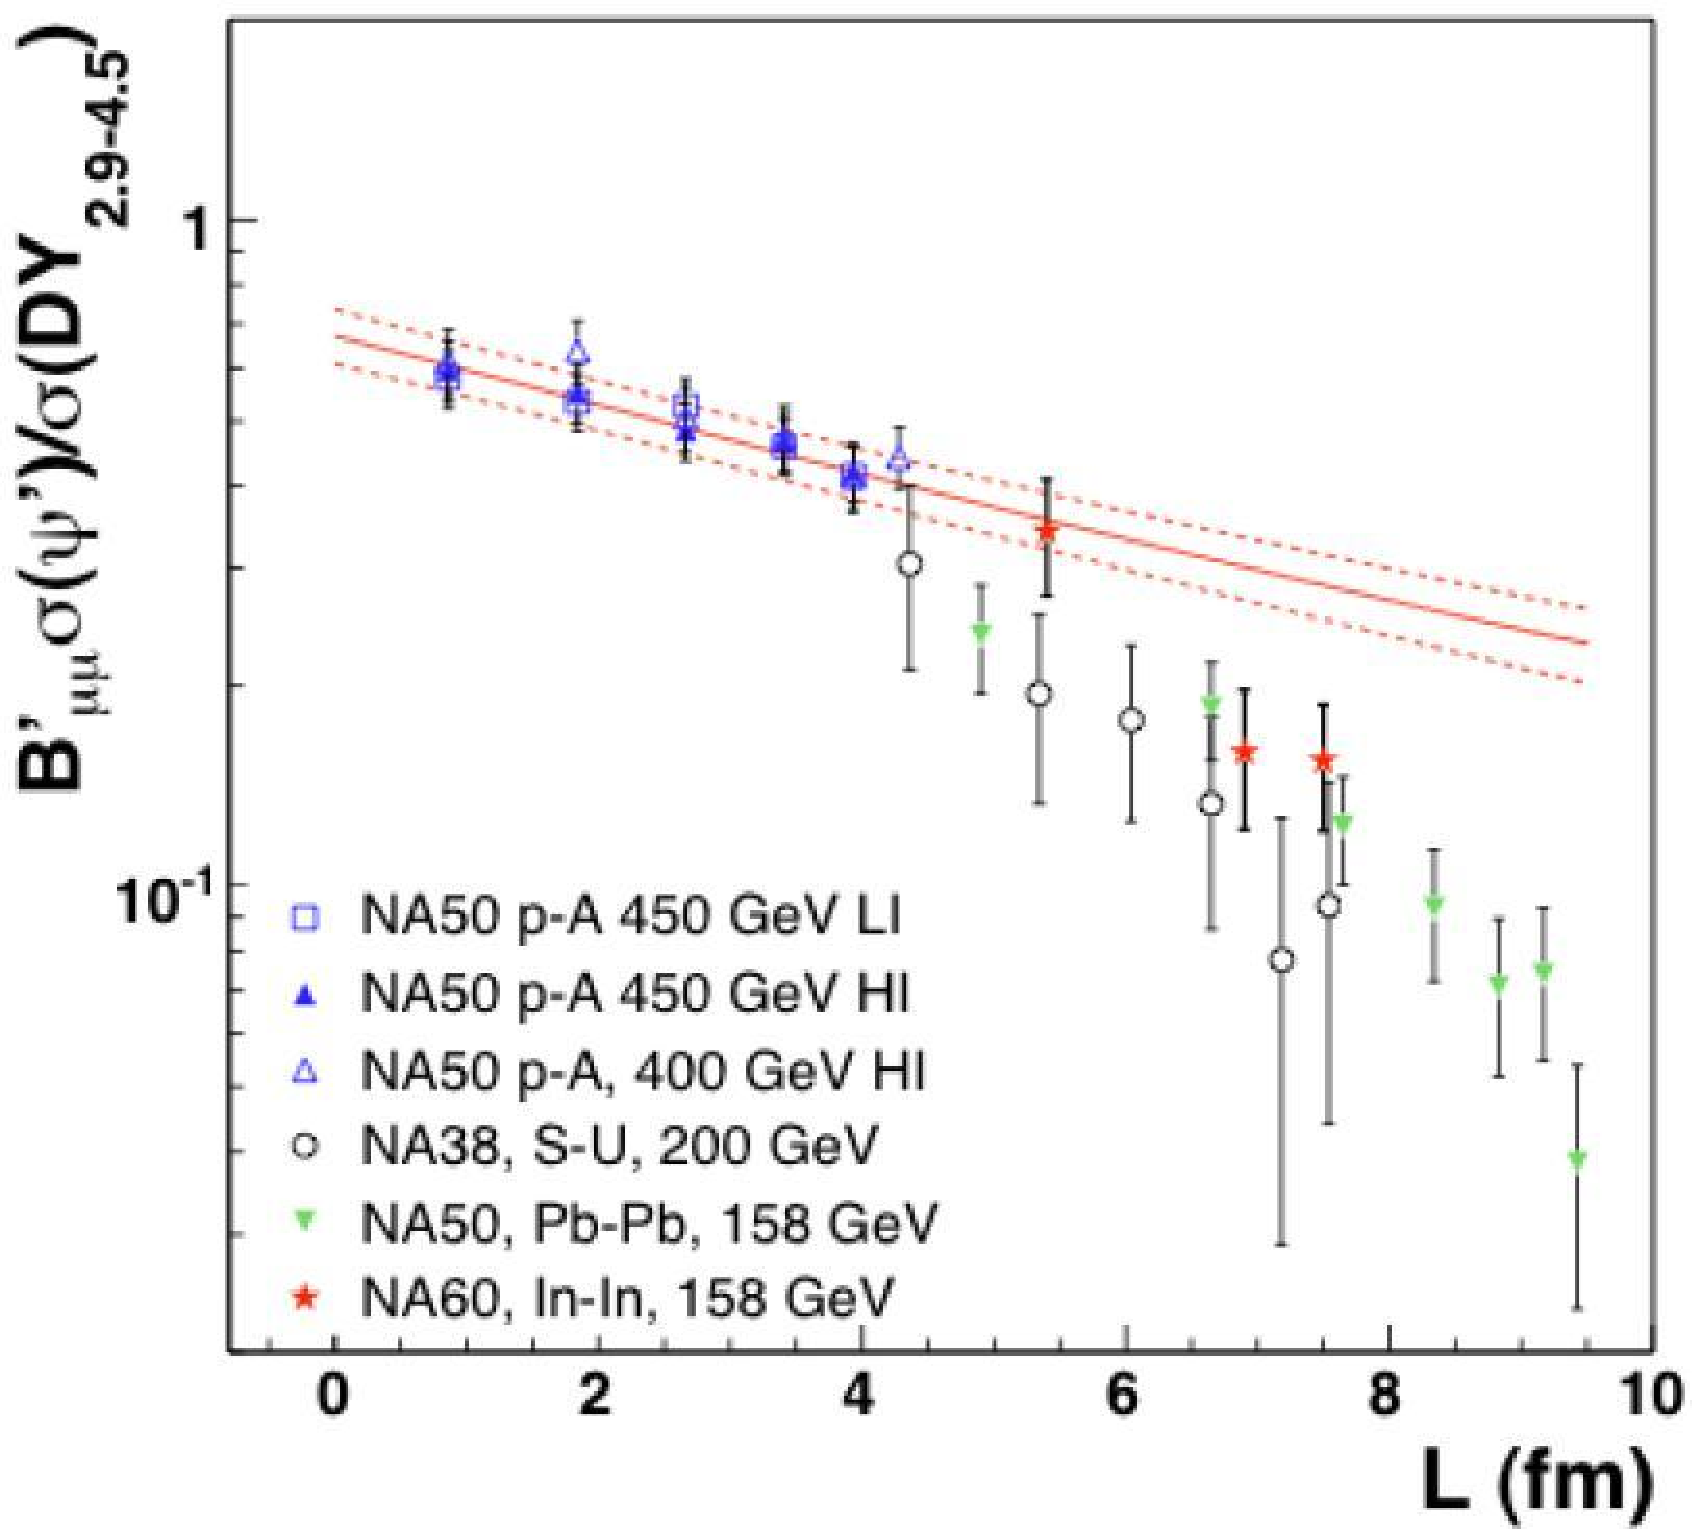
\includegraphics[width=\smallfigwidth]{chap_QuarkoniaSurvey_figures/SPS_Psi_218_2}
  \caption[PsiNA50NA60]{The ratio between cross section of $\psi^{'}$ times the branching into
    muons (B$_{\mu^{+}\mu^{-}}$) and the cross section of Drell$-$Yan reference process as measured
    by the NA50 and NA60 at various energies and in different collisional systems}
  \label{fig:PsiAtSPSNA50NA60}
\end{figure}


\begin{figure}
  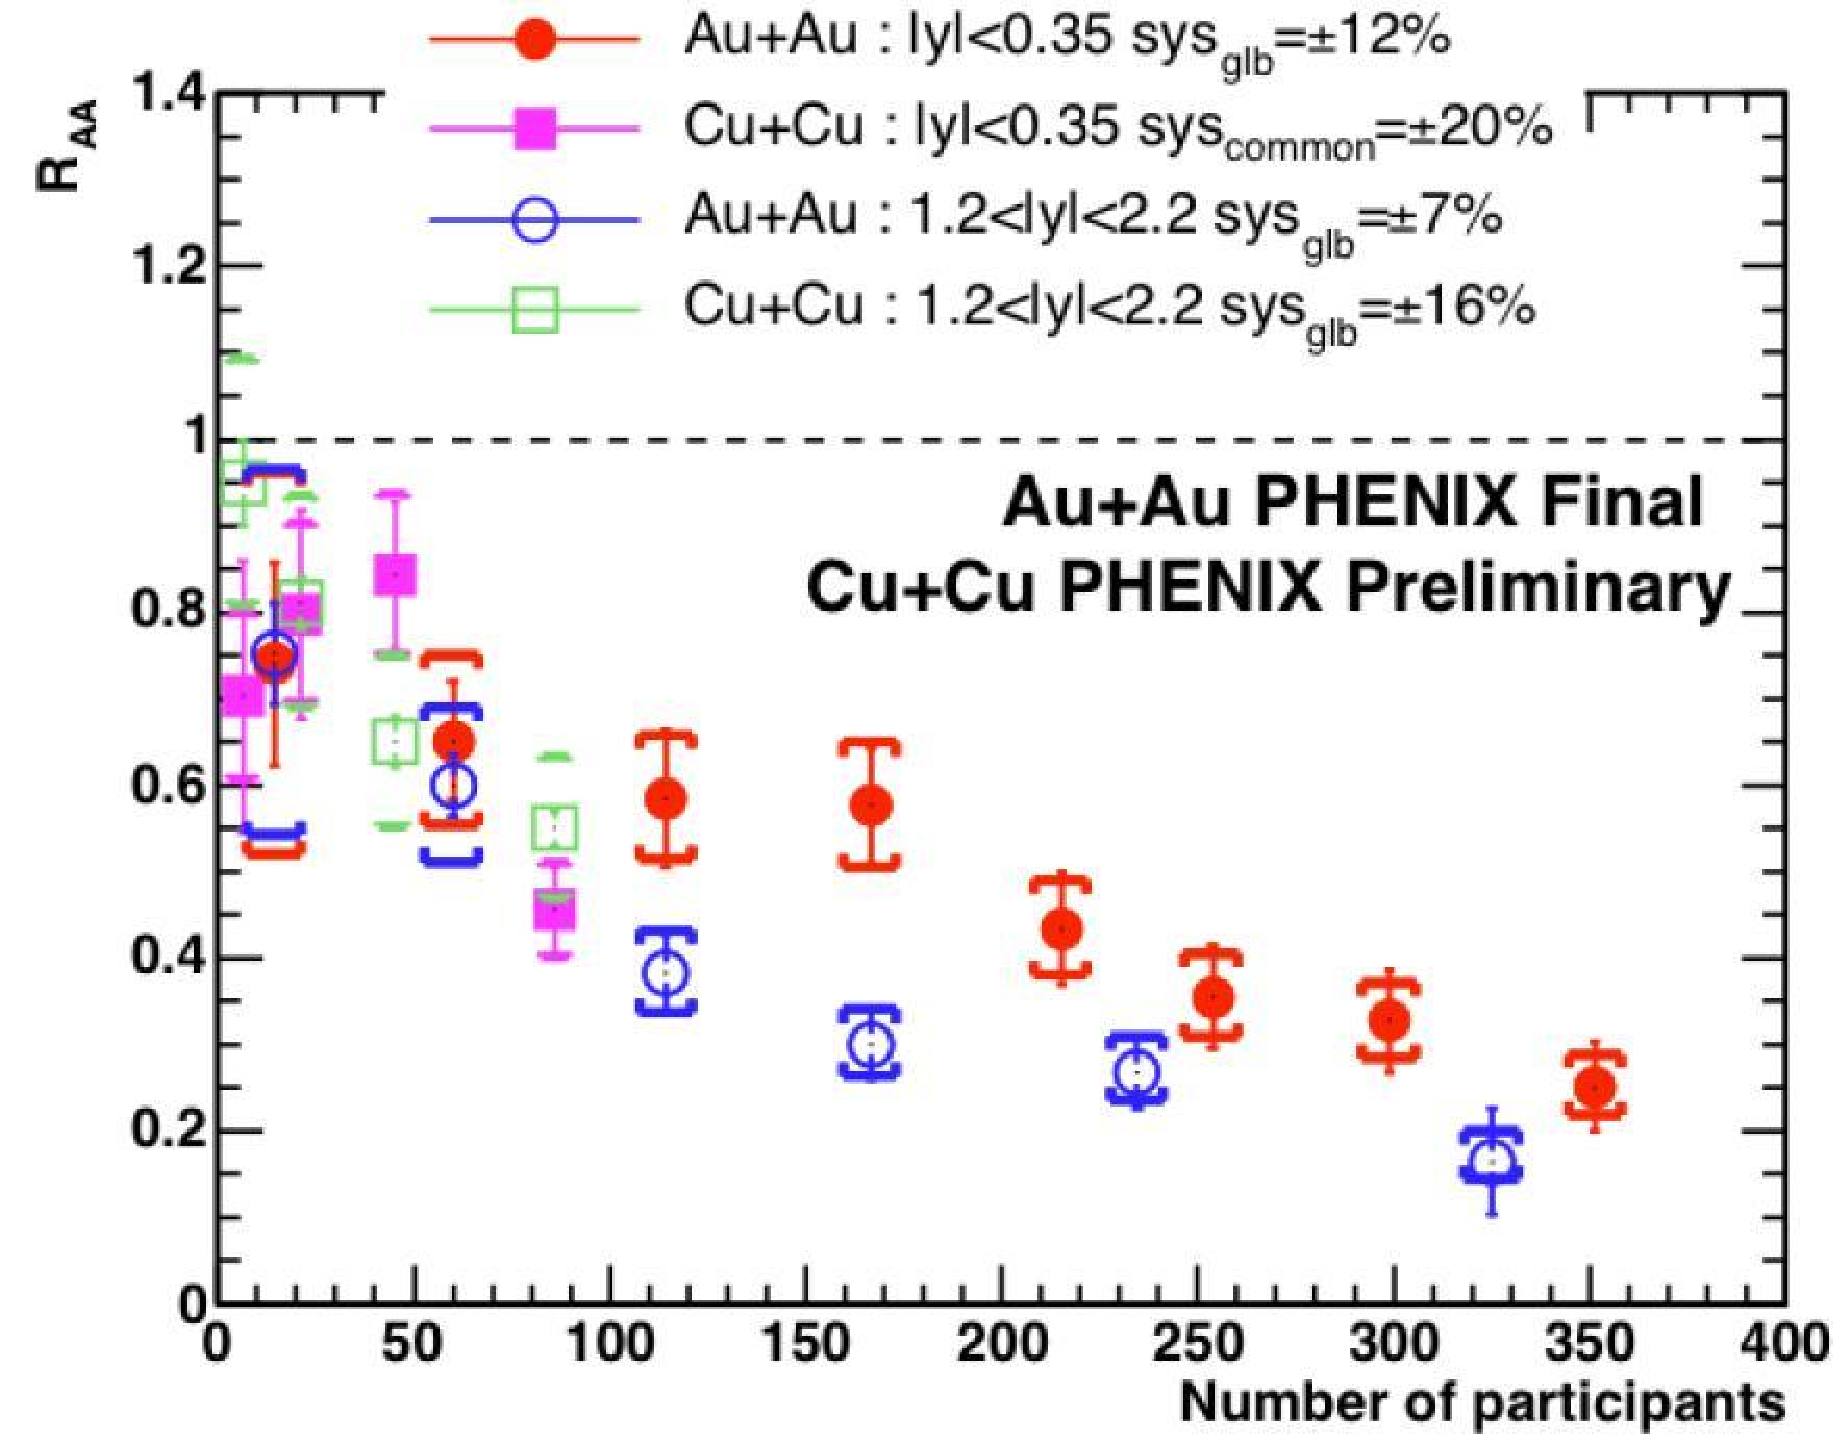
\includegraphics[width=\hugefigwidth]{chap_QuarkoniaSurvey_figures/RHIC_JPsi_219_1}
  \caption[JPsiRHICPhenix]{R$_{AA}$ as a function of Npart measured by PHENIX in Au$-$Au (in circles) and Cu$-$Cu (in squares) \cite{Phenix2}.}
   \label{fig:JPsiAtPHENIX1}
\end{figure}


\begin{figure}
  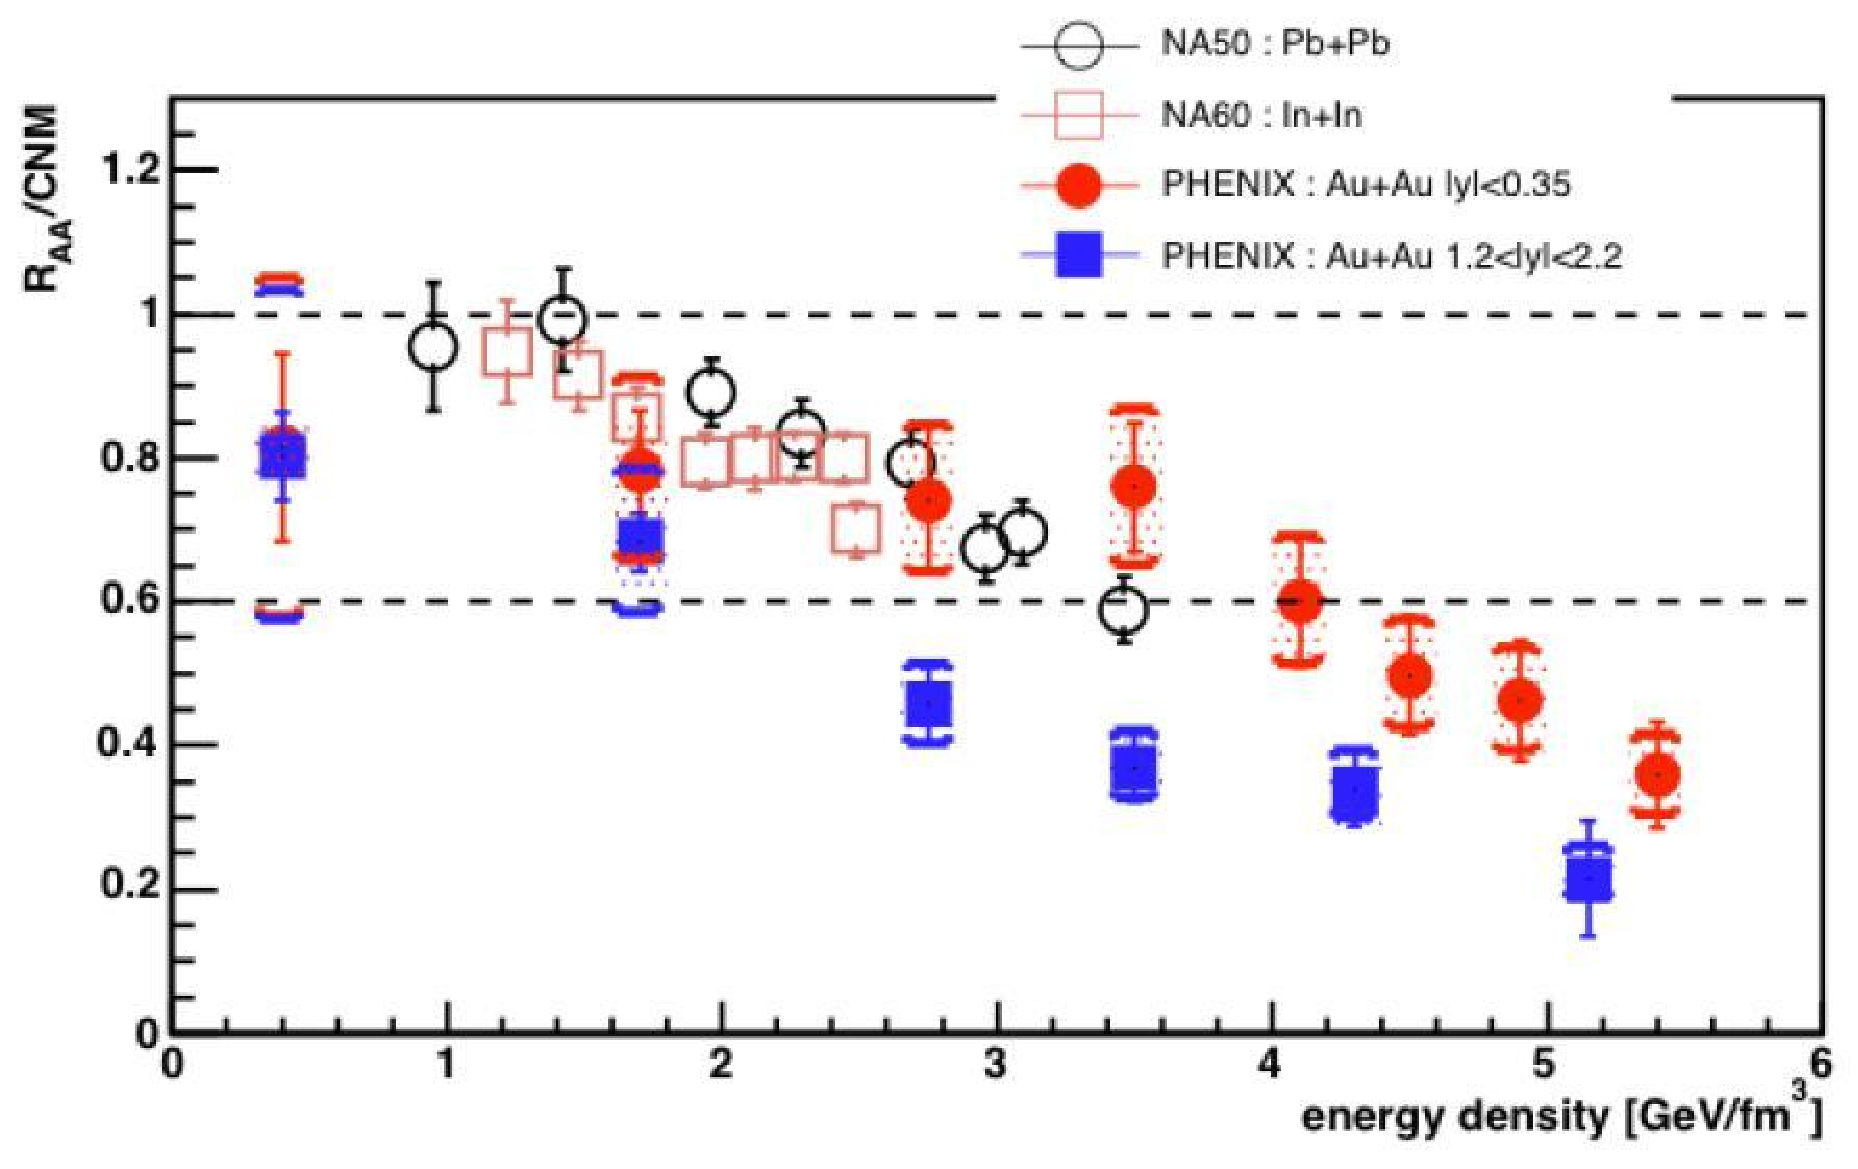
\includegraphics[width=\hugefigwidth]{chap_QuarkoniaSurvey_figures/RHIC_JPsi_219_2}
  \caption[JPsiRHICPhenix2]{R$_{AA}$/CNM as a function of the Bjorken estimate of the energy
     density. The RHIC data ($\sqrt{s_{NN}}$ = 200 GeV) is compared to SPS (17.3 GeV)
     measurements performed by NA50 and NA60 [70]. PHENIX estimates the cold nuclear matter 
     effects from measurements on d$-$Au, while the NA50 and NA60 rely on theoretical calculations.}
   \label{fig:JPsiAtPHENIX2}
\end{figure}

%\subsubsection{J/$\psi$ suppression at STAR}

\subsubsection{$\Upsilon(nS)$ suppression at RHIC}
STAR experiment at RHIC measure high p$_T$ J/$\psi$ and $\Upsilon$ states. 
Due to small production cross-section of b quark at 200 GeV, total yield 
of $\Upsilon$ is very small. STAR measure $\ee$ pairs ar mid rapidity $(|y| \leq 0.5)$. The unlike sign invariant
mass distribution, after subtracting like sign background is shown in Figure~\ref{fig:YinSTAR}:left. The measured yield
contain $\Upsilon$ signal as well as background from Drell$-$Yan and semileptonic decay of open beauty mesons.
The line-shape of the $\Upsilon$(1S+2S+3S) was parameterized with three crystal ball functions representing the successive states.
Different $\Upsilon$ states can not be seperated because of poor mass resolution as shown in Figure~\ref{fig:YinSTAR}:left.  
Measured $\Upsilon$ yield is devided in to three centrality bins: 0 $\%$ to 10$\%$, 10$\%$ to 30$\%$, and 30$\%$ to 60$\%$. 
R$_{AA}$ for the three centrality bins is shown in Figure~\ref{fig:YinSTAR}:right.
The results are compared to a model \cite{StrickLand} which incorporates lattice-based QCD calculations with a hydrodynamic
model of expansion and cooling. 
%[2] M. Strickland, D. Bazow arXiv:1112.2761v4,

\begin{figure}
  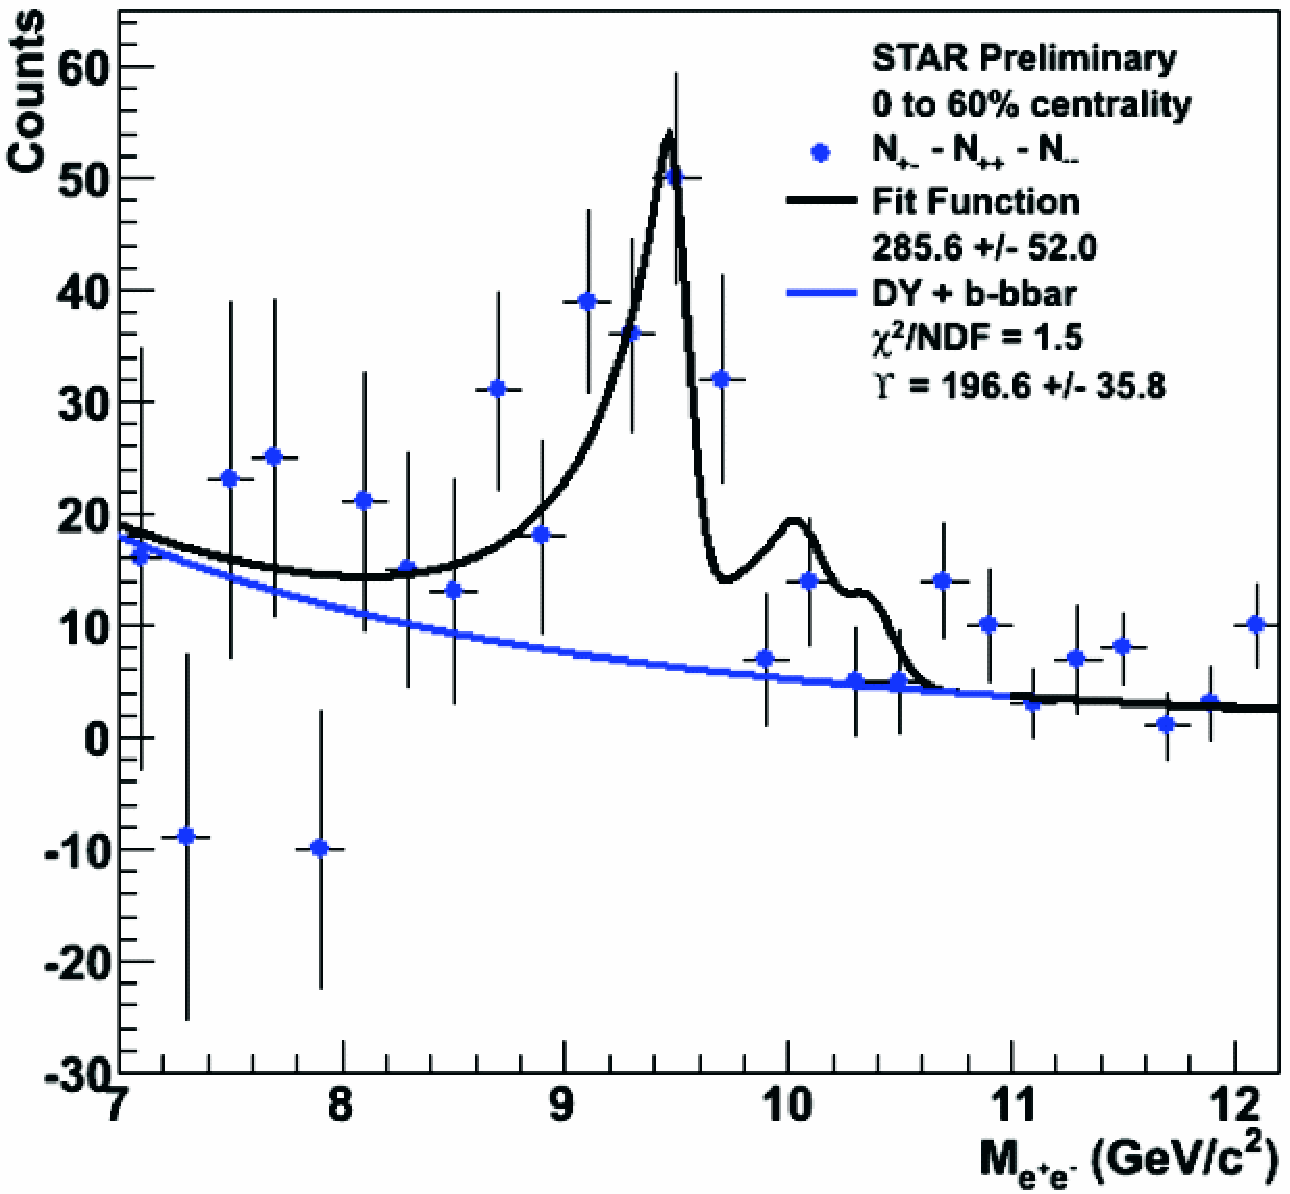
\includegraphics[width=\smallfigwidth]{chap_QuarkoniaSurvey_figures/YStar2011_InvMass}
  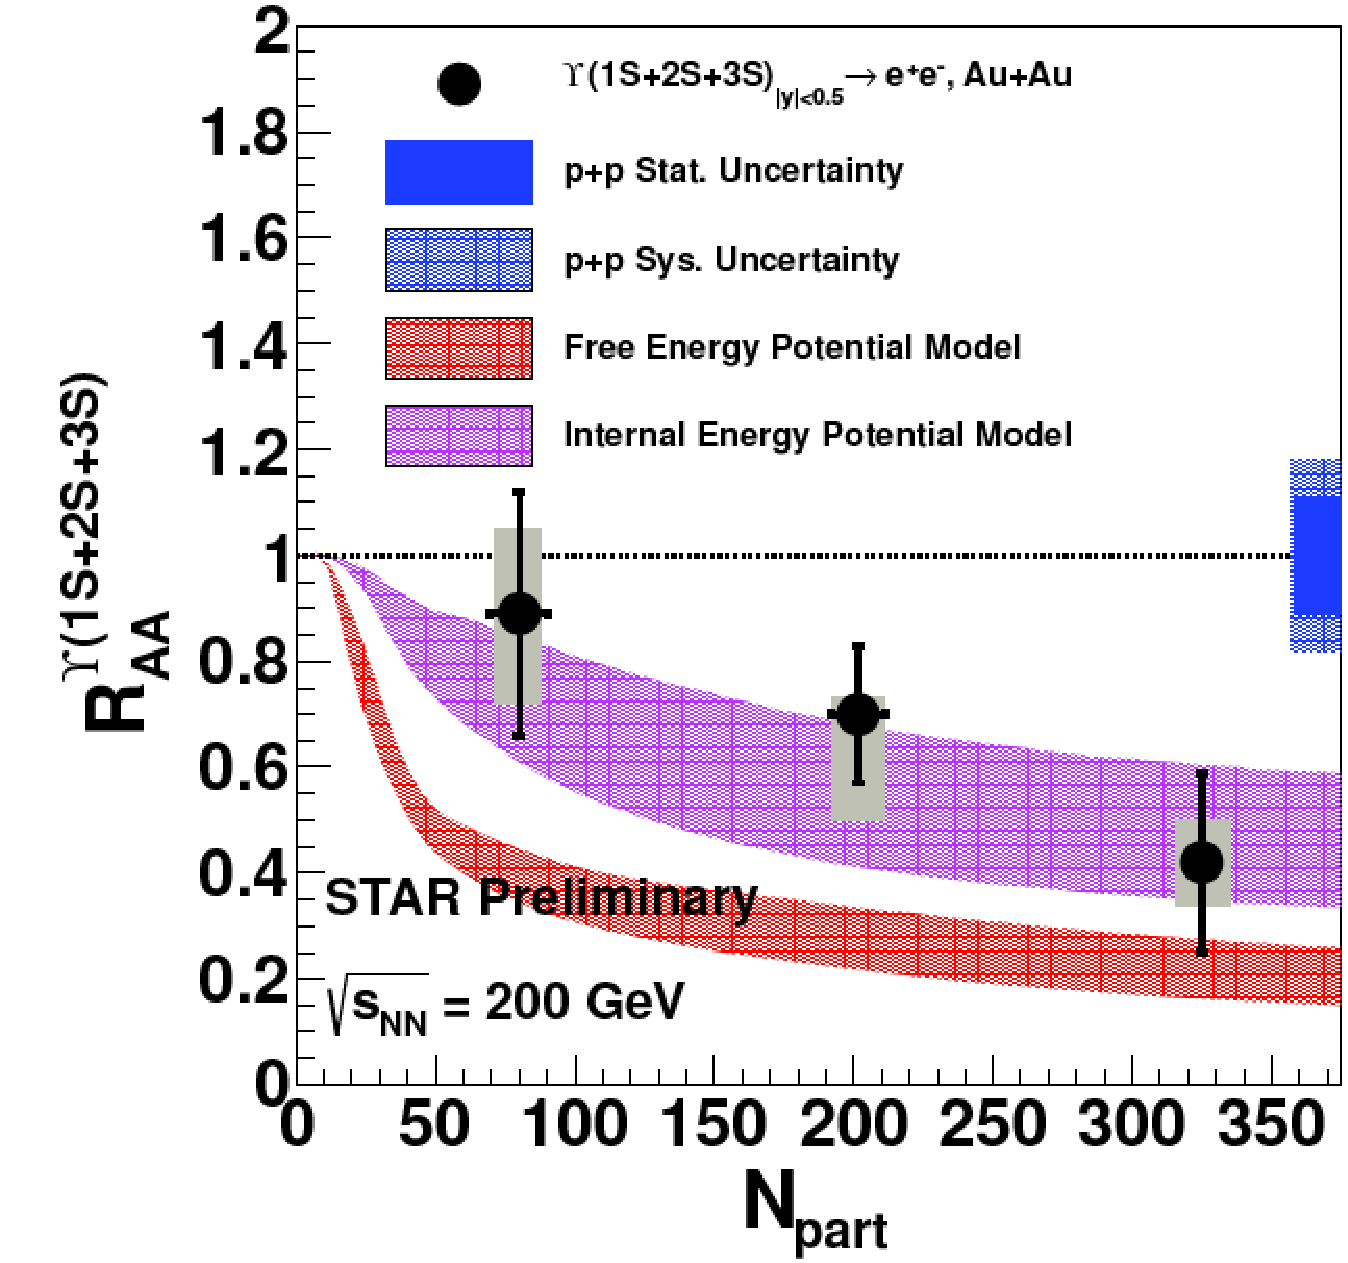
\includegraphics[width=\smallfigwidth]{chap_QuarkoniaSurvey_figures/YStar2011}
  \caption[]{left:$\ee$ pairs as measured in STAR detector at RHIC in 0$\%$-60$\%$ centrality class. The blue curve is the combination of Drell$-$Yan and b $\overline {b}$ 
    background. The black curve includes the Upsilon signal also. right: R$_{AA}$for 2010 Au+Au compared to 2009 p+p. The magenta and orange curves are theoretical 
    predictions using a combination of lattice-based QCD and hydrodynamical expansion and cooling \cite{Star12}.}
  \label{fig:YinSTAR}
\end{figure}




\begin{figure}
  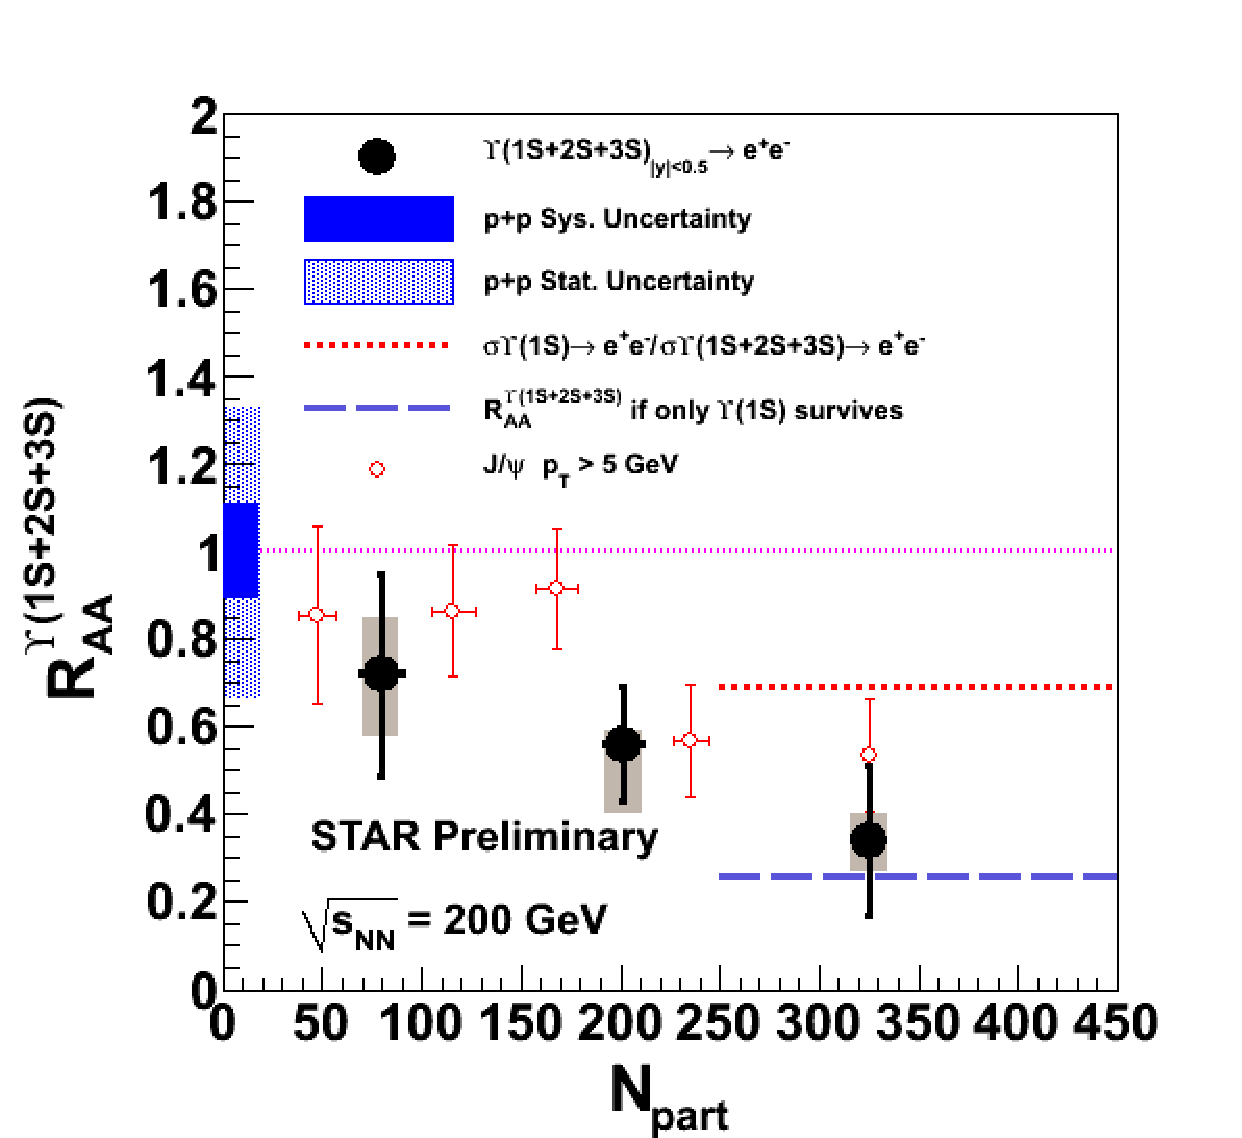
\includegraphics[width=\mediumfigwidth]{chap_QuarkoniaSurvey_figures/YStar2011_JPsiCompare}
  \caption[]{R$_{AA}$ for $\Upsilon(1S+2S+3S)$  versus centrality measured by STAR experiment at RHIC. The solid black points are the $\Upsilon$ R$_{AA}$. 
    The red open points are the high p$_T$ J/$\psi$ results from STAR. $\Upsilon$ R$_{AA}$ is compariable to J/$\psi$ in most central collisions.\cite{Star11}}
  \label{fig:YinSTAR2}
\end{figure}

Figure \ref{fig:YinSTAR2} shows $\Upsilon\,R_{AA}$ compared with high p$_T$ J/$\psi$ measured by STAR. A clear trend versus centrality can be seen in this graph.
The red dotted line is the ratio of the total cross-section of $\Upsilon$(1S)/$\Upsilon$(1S+2S+3S). The purple dashed line is the ratio of only the direct 
$\Upsilon$(1S) cross-section over the total $\Upsilon$(1S+2S+3S) cross-section. $\Upsilon$ R$_{AA}$ is compariable to J/$\psi$ in most central collisions. 

